    \documentclass[preprint,12pt,authoryear]{elsarticle}

\usepackage{graphicx}
\usepackage{amsfonts,amsmath}
\usepackage{amssymb,amsthm}
\DeclareMathOperator*{\argmin}{arg\,min}
\usepackage{dsfont}
\usepackage{longtable}
\usepackage{xcolor}
\usepackage{hyperref}
\usepackage{lineno}
\usepackage{booktabs}
\usepackage{microtype}
\usepackage{tabularx}
\usepackage{threeparttable}
%\usepackage{refcheck}
% TikZ removed — figures pre-rendered as PNG for faster compilation

% custom commands
\newcommand{\PD}{\text{PD}}
\newcommand{\DF}{\text{DF}}
\newcommand{\CL}{\text{CL}}
\newcommand{\ECL}{\mathbb{E}[\text{CL}]}
\newcommand{\ICR}{\text{ICR}}
\newcommand{\EBIT}{\text{EBIT}}
\newcommand{\IE}{\text{IE}}
\newcommand{\MC}{\text{MC}}
\newcommand{\FS}{\text{FS}}
\newcommand{\RR}{\text{RR}}

\tolerance = 3000

\journal{Natural Hazards Research}

\begin{document}

\begin{frontmatter}

\title{A duration-dependent flood depth-damage function calibrated using FEMA NFIP claims from three U.S. hurricanes}

\author[airi]{Ivan Novikov\corref{cor1}\fnref{fn1}}
\ead{ivan.novikov@iccda.io}
\author[airi]{Nikita Lazarichev\fnref{fn1}}
\author[airi]{Denis Ayvazov}
\author[airi]{Aleksandr Popov}
\author[msu]{Yuriy Dorn}
\author[msu]{Roman Sultimov}
\author[interdata]{Aleksandr Volkov}
\author[msu]{Andrey Osipsov}
\author[interdata]{Yury~Maximov}

\cortext[cor1]{Corresponding author}
\fntext[fn1]{Ivan Novikov and Nikita Lazarichev contributed equally to this work.}

\address[airi]{Moscow Research Institute of Artificial Intelligence, Moscow, Russia}
\address[msu]{Moscow State University, Moscow, Russia}
\address[interdata]{Interdata, Astana, Kazakhstan}

\begin{abstract}
\textbf{Background:} Standard depth-damage functions used in climate risk assessment---including those underpinning CLIMADA and JRC impact models---treat flood damage as an instantaneous function of water depth, ignoring the duration of inundation.

\textbf{Methods:} We extend the generalised logistic (Richards) damage function with duration-dependent parameters and calibrate it on 295{,}637 flood insurance claims from the FEMA National Flood Insurance Program (OpenFEMA snapshot 2026-05-09), spanning three major US hurricanes: Sandy (2012, $\sim$36\,h), Harvey (2017, $\sim$288\,h), and Katrina (2005, $\sim$120\,h). To bridge the residential calibration to non-residential assets, we introduce a sector adjustment multiplier $\kappa$ calibrated on 82{,}650 NFIP non-residential claims grouped by building stories and insurance coverage, combined with a coverage-gradient extrapolation to corporate scale.

\textbf{Results:} Prolonged flooding increases structural damage by a factor of 2.6$\times$ at the same depth, and this effect operates primarily through a shift in the curve's inflection point ($\lambda_a = 0.49$), while the fundamental shape of the damage function remains universal across events. The calibrated model reduces mean absolute error by about 50\% relative to JRC depth-damage curves and achieves Spearman $\rho = 0.949$ ($p < 0.001$) against actual financial damage across 301 ZIP codes. Out-of-sample validation on 24 companies across six flood events yields a median predicted-to-actual ratio of 0.90$\times$ (23/24 within 0.4--2.5$\times$), with no corporate loss disclosures entering the calibration.

\textbf{Conclusions:} Duration is a first-order determinant of flood damage that existing vulnerability frameworks systematically miss. We demonstrate the full pipeline on Archer Daniels Midland's 12 flood-exposed Midwest facilities, producing facility-level loss estimates with duration effects, CapEx/OpEx decomposition, and insurance offsets. The framework translates physical damage into shifts in probability of default via an interest coverage ratio approach, enabling direct integration with banks' internal credit risk models.

\end{abstract}

\begin{keyword}
flood duration \sep damage function \sep FEMA NFIP \sep flood vulnerability \sep hazard loss assessment \sep non-residential assets
\end{keyword}

\end{frontmatter}

\linenumbers



\section{Introduction}
\label{sec: intro}
Flood damage assessment is a cornerstone of physical climate risk quantification for financial institutions. The Basel Committee on Banking Supervision~\cite{basel2021a, basel2021b} identifies data scarcity  --  particularly the lack of paired hazard-loss observations for damage function calibration  --  as the single most critical gap in the physical risk assessment pipeline. Existing depth-damage functions, such as those maintained by the Joint Research Centre~\cite{huizinga2017global} and the US Army Corps of Engineers~\cite{usace2003}, treat damage as an instantaneous function of water depth. These functions underpin widely used platforms including CLIMADA~\cite{aznar2019climada} and form the basis for regulatory stress tests~\cite{ecb2025stress}. Yet they ignore a physically obvious variable: the duration of inundation. A flood that recedes in hours causes fundamentally different damage from one that persists for weeks, through material saturation, mould growth, electrical system failure, and structural weakening.

This omission has measurable consequences. Using 295{,}637 cleaned FEMA NFIP claims from three major US hurricanes, we show that standard JRC depth-damage functions systematically underpredict damage by about 15 percentage points for prolonged events -- a bias that propagates directly into credit risk estimates for flood-exposed companies.

\subsection{Contribution}

This paper makes three contributions:

\begin{enumerate}
    \item We extend the generalised logistic (Richards) damage function with a \textit{duration-dependent formulation} in which the curve's inflection point, onset speed, and asymmetry depend continuously on hazard duration. We calibrate the seven parameters jointly on 295{,}637 FEMA NFIP flood insurance claims spanning Hurricanes Sandy (36\,h), Harvey (288\,h), and Katrina (120\,h). The key empirical finding is that duration primarily affects damage through inflection point shift ($\lambda_a = 0.49$), while curve shape parameters are not significantly non-zero in the three-event calibration ($\lambda_Q \approx 0$, $\delta_\nu \approx 0$); this conclusion is, however, limited by the fact that the calibration spans only three distinct event-level duration values.

    \item We introduce a \textit{sector adjustment multiplier} $\kappa$ calibrated empirically from 82{,}650 NFIP non-residential claims, grouped by number of stories and insurance coverage. A coverage-gradient extrapolation bridges NFIP-scale commercial buildings to corporate-scale facilities without relying on corporate loss disclosures. Out-of-sample validation on 24 companies across six flood events yields a median predicted-to-actual ratio of $0.90\times$ (23/24 within 0.4--2.5$\times$).

    \item We demonstrate the \textit{full calibrated pipeline} on Archer Daniels Midland's 12 flood-exposed Midwest facilities, producing facility-level loss estimates with duration-dependent damage ratios, CapEx/OpEx decomposition, insurance offsets, and credit risk translation via an interest coverage ratio approach. The framework is modular: the credit risk translation module can employ alternative models (including the Merton structural model~\cite{merton1974pricing}) without changing the damage assessment.
\end{enumerate}

\subsection{Data requirements}

The framework requires: (i) asset locations and replacement values, obtainable from company filings; (ii) local flood hazard parameters (depth, duration), available from FEMA flood maps and hydrological models; (iii) financial statements (EBIT, debt, interest expenses) for credit risk translation. The damage function parameters are provided by our calibration and do not require company-specific fitting.

\subsection{Paper organisation}

Section~\ref{sec: lit review} reviews damage function literature and the calibration data gap. Section~\ref{sec: methods} presents the framework architecture, the duration-dependent Richards formulation, sector adjustment, and credit risk translation. Section~\ref{sec: empirical} describes the FEMA dataset, joint calibration, and four validation tests. Section~\ref{sec: adm} applies the calibrated pipeline to ADM. Section~\ref{sec: event study} presents the Hurricane Harvey event study. Section~\ref{sec: discussion} discusses findings and limitations. Section~\ref{sec: conclusion} concludes.


\section{Related Work}
\label{sec: lit review}
\paragraph{Depth-damage functions}
Depth-damage functions map a hazard intensity measure to a damage ratio (repair cost relative to replacement value) and are the primary tool for translating flood hazard into economic loss. In the flood context, inundation depth is the dominant intensity measure and serves as the primary input to these functions~\cite{merz2010review, huizinga2017global}; other intensity measures such as flow velocity and inundation duration are secondary but can be material for specific flood types and asset classes~\cite{merz2010review}. The most widely used functions originate from engineering studies by the US Army Corps of Engineers~\cite{usace2003}, which developed stage-damage curves for residential structures based on expert judgement and post-disaster surveys. The Joint Research Centre of the European Commission~\cite{huizinga2017global} extended this approach globally, producing continent-specific depth-damage curves for residential, commercial, and industrial assets. These JRC functions are the default vulnerability module in CLIMADA~\cite{aznar2019climada}, the open-source platform developed at ETH Zurich for probabilistic natural catastrophe impact assessment.

A common limitation of these functions is the absence of a duration parameter. All standard depth-damage curves treat damage as an instantaneous mapping from water depth to loss, implicitly assuming that a flood of one metre depth produces the same damage whether it recedes in two hours or persists for two weeks. This assumption is physically unrealistic: prolonged inundation causes additional degradation through water absorption by building materials, mould colonisation, corrosion of electrical and mechanical systems, and progressive structural weakening~\cite{merz2010review}. Several engineering studies have documented the duration effect qualitatively and incorporated it into multi-variable damage models alongside depth and flow velocity~\cite{merz2010review}. Recent work has begun to formalise depth-damage relationships for the built environment~\cite{pistrika2014flood} and to extend them toward probabilistic vulnerability and functionality-loss frameworks~\cite{pandey2026urban, forte2025flash, gautam2022unzipping}. Post-event field surveys further document the breadth of damage mechanisms activated during extreme flood episodes~\cite{santangelo2021landslides, thapa2020catchment, santo2016post, chinh2016mekong}. However, quantitative calibration of a duration-dependent parametric function on large-scale insurance claims data has been lacking. This is the gap addressed by the present paper.

\paragraph{Calibration data gap}
The Basel Committee~\cite{basel2021a, basel2021b} and industry surveys~\cite{unepfi2025bridging} consistently identify data scarcity as the primary obstacle to developing reliable physical risk models. Damage function calibration requires paired observations of hazard intensity and economic loss at the building or asset level --- data that are rarely available outside the insurance sector. The FEMA National Flood Insurance Program (NFIP) represents one of the few large-scale sources of such data, with millions of individual claims containing water depth, payout, and building characteristics. Machine learning approaches have demonstrated the potential for multi-variable flood damage estimation when richer hazard and building-characteristic data are available, including gradient-boosted and causal ML models applied to residential properties~\cite{museru2025improving, museru2024advancing} and ensemble deep learning models for flood forecasting~\cite{kordani2024improving}. To our knowledge, this paper presents the first systematic calibration of a parametric damage function with duration dependence on NFIP data at the scale of 295{,}637 claims.

\paragraph{Flood risk across infrastructure sectors}
Flood risk assessment extends beyond residential properties to critical infrastructure and community-scale systems. Studies of wastewater treatment facilities~\cite{nazari2022hydrodynamic, sun2021comprehensive}, coastal structures~\cite{fahad2020coupled, fahad2022decision}, and earthen infrastructure~\cite{motamedi2018quantitative} document sector-specific vulnerability patterns. Economic resilience analyses at the community scale~\cite{nazari2025small} complement asset-level damage estimation by capturing wider socioeconomic disruption. These application contexts motivate the sector adjustment module ($\kappa$) introduced in Section~\ref{ssec: sector}.

\paragraph{Physical climate risk and credit}
A growing body of research demonstrates that physical climate hazards materially affect corporate creditworthiness. Cathcart et al.~\cite{cathcart2026rain} find that temperature and precipitation anomalies increase default probabilities for small firms by 32--87 basis points per standard deviation. Abinzano et al.~\cite{abinzano2026physical} provide global evidence that physical climate risk increases banks' credit risk, with effects concentrated in weakly capitalised institutions. The Bank for International Settlements~\cite{bis2025physical} argues that physical risks have evolved from a niche concern into a systemic risk factor requiring integration into credit risk models.

On the methodology side, Moody's Analytics~\cite{bocchio2023quantifying} and MSCI~\cite{msci2024transition} have developed proprietary frameworks that translate climate scenarios into changes in expected default frequency, using top-down GDP allocation and structural credit models. Bourgey et al.~\cite{bourgey2025climacred} contribute a micro-founded theoretical model linking default probabilities to NGFS scenarios. However, these approaches rely on aggregate damage estimates rather than empirically calibrated, asset-level damage functions --- precisely the gap that our calibration addresses.

\paragraph{Sector-specific vulnerability}
The distinction between residential and commercial/industrial vulnerability is well documented in the flood damage literature~\cite{merz2010review, huizinga2017global}. Commercial buildings typically have higher floor elevations, more robust construction, and operational redundancy that reduces effective damage ratios. However, quantitative estimates of the residential-to-commercial damage ratio---what we term the sector adjustment multiplier $\kappa$---are sparse and typically based on engineering judgement rather than loss data. Our approach calibrates $\kappa$ empirically from 82{,}650 NFIP non-residential claims grouped by observable building characteristics, providing a data-driven alternative to expert-based estimates.


\begin{longtable}[c]{l|p{10cm}}
$\DF$ & Damage Function (ratio of repair cost to replacement value) \\
$\PD$, $\mathbf{P}_D$ & Probability of default\\
$\Delta \PD_C$ & Shift in probability of default driven by climate risks\\
$\CL, \ECL$ & Climate Loss, Expected Climate Loss \\
$\ICR, \ICR_C$ & Interest Coverage Ratio, Climate-adjusted ICR \\
$\EBIT$ & Earnings Before Interest and Taxes \\
$\IE$ & Interest Expenses \\
$\RR$ & Recovery Rate \\
$\kappa$, $\kappa_{\text{claims}}$, $\kappa_{\text{total}}$ & Sector adjustment multiplier: claims-based and total (including $\rho$) \\
$\rho_{\text{gradient}}$ & Coverage-gradient resilience factor for corporate-scale facilities \\
$\tau$ & Hazard duration (hours) \\
$h$ & Flood depth (metres) \\
$r$ & Risk-free rate\\[1ex]
\caption{Notation}
\end{longtable}


\section{Framework and Methodology}
\label{sec: methods}
Our approach follows a three-stage pipeline aligned with the BCBS transmission framework~\cite{basel2021a}: hazard characterisation $\to$ damage estimation $\to$ credit risk translation (Fig.~\ref{fig: scheme}).

\begin{figure}[ht]
\centering
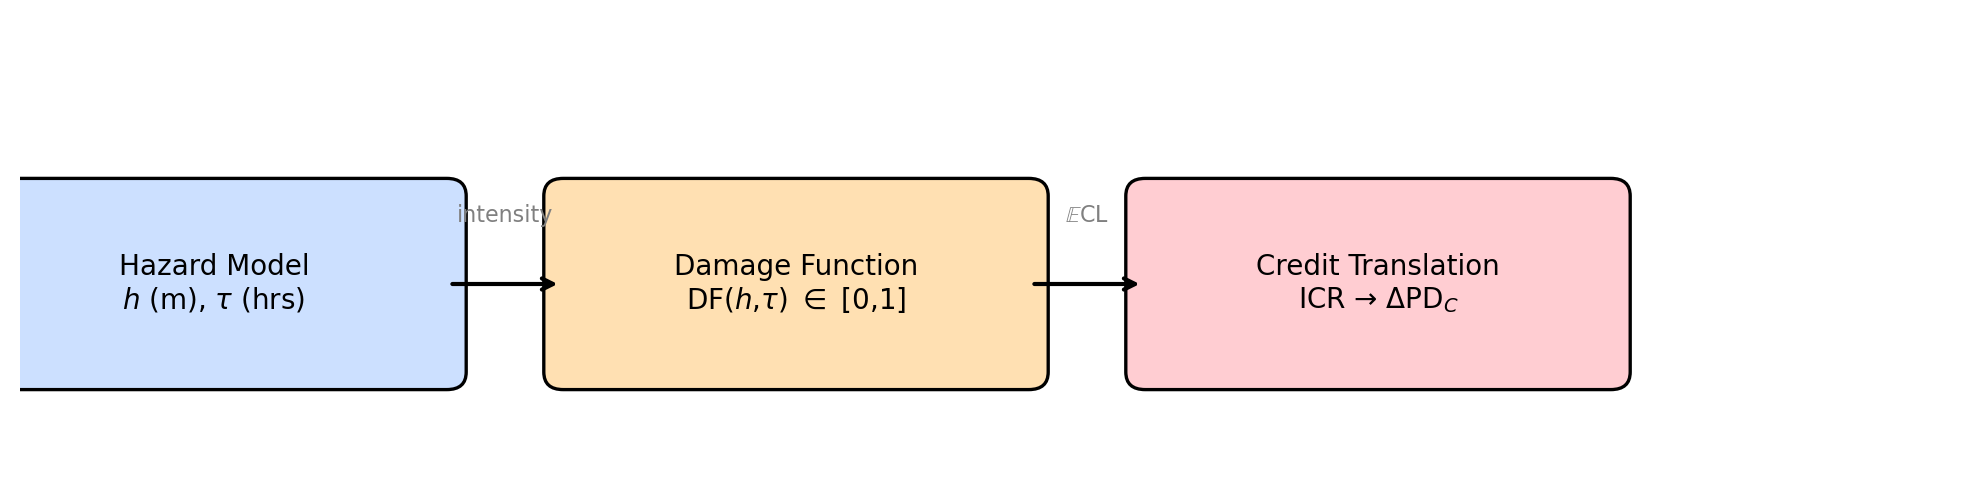
\includegraphics[width=0.85\textwidth]{Content/Images/pipeline_scheme.png}
\caption{Three-stage pipeline: hazard intensity is converted to a damage ratio via the parametric damage function (Sections~\ref{ssec: damage function}--\ref{ssec: sector}), then translated into a PD shift (Section~\ref{ssec: pd shift}).}
\label{fig: scheme}
\end{figure}

The \textit{hazard characterisation} stage provides the probability and intensity of physical hazards at each asset location. For floods, the key variables are water depth $h$ (metres) and inundation duration $\tau$ (hours), obtained from FEMA flood zone maps, hydrological models, or scenario-based projections. The \textit{damage estimation} stage converts hazard intensity into a damage ratio $\DF \in [0,1]$ via a parametric damage function. This is the primary methodological contribution of the paper: we extend the standard Richards function with duration dependence and calibrate it empirically (Sections~\ref{ssec: damage function}--\ref{ssec: sector}). The \textit{credit risk translation} stage converts expected monetary losses into a shift in probability of default $\Delta PD_C$, using the interest coverage ratio approach described in Section~\ref{ssec: pd shift}. This module is deliberately kept simple and replaceable --- more sophisticated models, including multi-ratio logistic regression~\cite{altman2007modelling, ohlson1980financial}, the Merton structural model~\cite{merton1974pricing}, or other approaches, can substitute for it without affecting the upstream damage estimation.

The data flow for a multi-location company proceeds as follows (Fig.~\ref{fig: dataflow}): asset locations are mapped to local hazard parameters, damage ratios are computed per facility, and losses are aggregated to the company level before credit translation.

\begin{figure}[ht]
\centering
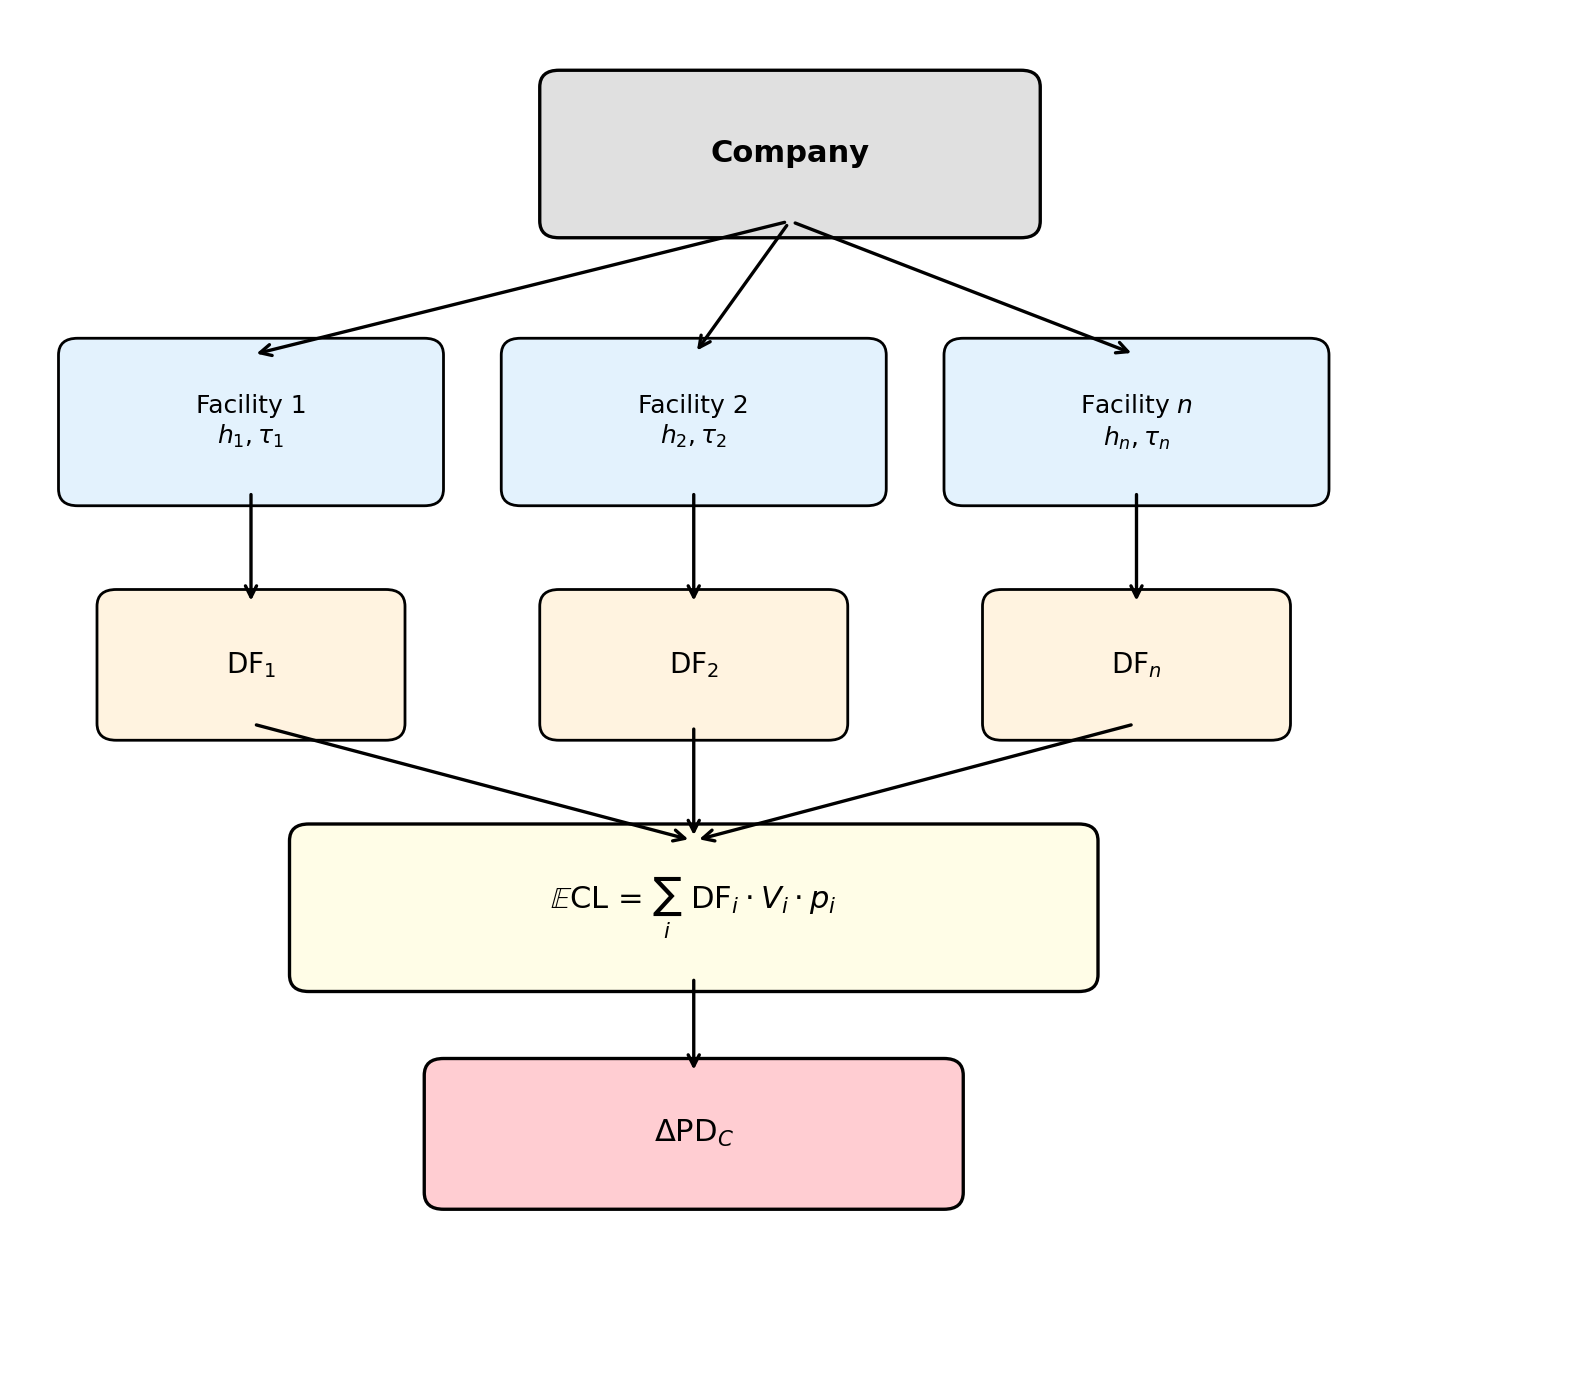
\includegraphics[width=0.55\textwidth]{Content/Images/dataflow_diagram.png}
\caption{Data flow for a multi-location company: each facility's hazard parameters are converted to a damage ratio, losses are aggregated by replacement value $V_i$ and event probability $p_i$, then translated into a PD shift.}
\label{fig: dataflow}
\end{figure}


\subsection{Parametric Damage Function} \label{ssec: damage function}
The damage function maps hazard intensity to a damage ratio $\DF \in [0,1]$, representing the repair cost as a fraction of replacement value. We adopt the generalised logistic (Richards) function as our parametric form:

\begin{equation}
    Y(x) = A + \frac{K - A}{\left( C + Q \exp{[-B(x - a)]} \right)^{\frac{1}{\nu}}}
    \label{eq: logistic function}
\end{equation}
with $A = 0$, $K = 1$, $C = 1$ for damage ratios bounded in $[0,1]$. The remaining parameters have clear physical interpretations: $B$ controls the steepness of the damage curve (how rapidly damage increases with depth); $a$ sets the inflection point (the depth at which damage reaches approximately 50\%); $Q$ affects onset speed (how quickly damage departs from zero); and $\nu$ controls asymmetry (whether damage accelerates faster at low or high depths).

\begin{figure}[ht]
\centering
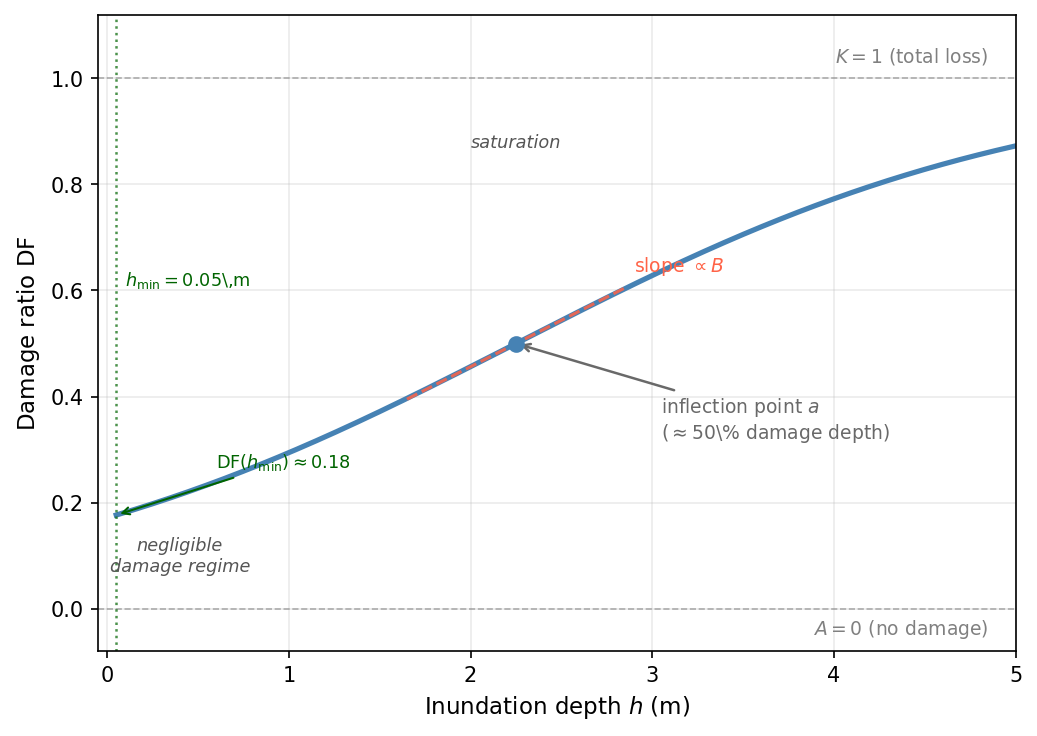
\includegraphics[width=0.75\textwidth]{Content/Images/richards_schematic.png}
\caption{Schematic Richards damage function: the S-shaped curve transitions from negligible damage at low depths through a steep transition (controlled by $B$) centred at inflection point $a$ to saturation near total loss. Note: the Richards function approaches $\DF = 0$ only asymptotically as $h \to -\infty$; at $h = 0$ the function takes a small positive value ($\approx 0.19$ for the calibrated parameters), reflecting the minimum-damage floor below which flooding is not practically relevant. Curves are plotted from $h_{\min} = 0.05$\,m.}
\label{fig: damage function}
\end{figure}

The Richards function has sufficient flexibility to capture the main features of empirical depth-damage relationships --- an initial low-damage regime, a rapid transition, and saturation near total loss --- while remaining parsimonious enough (four free parameters for a single-variable, instantaneous function) to avoid overfitting on noisy insurance claims data.

The calibration output is a parameter set $(a, B, Q, \nu)$ for each combination of hazard type and asset category:
\begin{equation*}
    \text{Category}_i, \text{ Hazard}_j : \quad (a_{ij}, B_{ij}, Q_{ij}, \nu_{ij})
    %\label{eq: calibration result}
\end{equation*}
In this paper, we calibrate for the flood--residential combination using FEMA data (Section~\ref{sec: empirical}) and bridge to commercial assets via the sector adjustment (Section~\ref{ssec: sector}).


\subsection{Duration-Dependent Extension} \label{ssec: duration}
The standard Richards function treats hazard intensity as instantaneous: a flood of depth $h$ produces damage ratio $\DF(h)$ regardless of whether the water recedes after two hours or persists for two weeks. This assumption is adequate for acute hazards such as hailstorms but significantly underestimates damage for prolonged flooding, where water contact duration drives additional degradation through material saturation, mould growth, electrical system failure, and structural weakening.

We extend the Richards function by making its parameters depend continuously on hazard duration $\tau$:

\begin{equation}
    \DF(h, \tau) = \frac{1}{\left(1 + Q(\tau) \exp\left[-B \cdot \left(\frac{h - F_{\min}}{F_s - F_{\min}} - a(\tau)\right)\right]\right)^{1/\nu(\tau)}}
    \label{eq: duration richards}
\end{equation}
where the duration-dependent parameters are:
    $a(\tau) = a_0 \cdot \exp\left(-\lambda_a \cdot \frac{\tau}{\tau_0}\right)$,
    $Q(\tau) = Q_0 \cdot \exp\left(-\lambda_Q \cdot \frac{\tau}{\tau_0}\right)$, 
    $\nu(\tau) = \nu_0 + \delta_\nu \cdot \ln\left(1 + \frac{\tau}{\tau_0}\right)$. 

Here $\tau_0 = 48$~hours is a reference duration scale, and $\lambda_a$, $\lambda_Q$, $\delta_\nu$ are duration sensitivity coefficients. The physical interpretation is:
\begin{itemize}
    \item $a(\tau)$ controls the inflection point: as duration increases, the ``50\% damage depth'' shifts toward shallower water, reflecting the empirical observation that prolonged shallow flooding causes damage comparable to brief deep flooding;
    \item $Q(\tau)$ controls onset speed: longer duration accelerates the transition from zero to significant damage;
    \item $\nu(\tau)$ controls curve asymmetry: prolonged events produce concave (fast-onset, slow-saturation) curves rather than the symmetric sigmoid of instantaneous events.
\end{itemize}

At $\tau = 0$, the function reduces exactly to the standard Richards form (Eq.~\ref{eq: logistic function}) with parameters $(B, Q_0, a_0, \nu_0)$, ensuring backward compatibility. The total number of calibratable parameters is seven: $(B, Q_0, a_0, \nu_0, \lambda_a, \lambda_Q, \delta_\nu)$.

The duration-dependent extension produces a continuous family of damage curves that transitions smoothly from a sigmoidal shape (instantaneous events) to a concave form (prolonged events). Fig.~\ref{fig:duration_curves} illustrates the effect: as $\tau$ increases, the inflection point shifts leftward (toward shallower depths), so that even moderate flooding causes substantial damage after prolonged inundation.

\begin{figure}[ht]
\centering
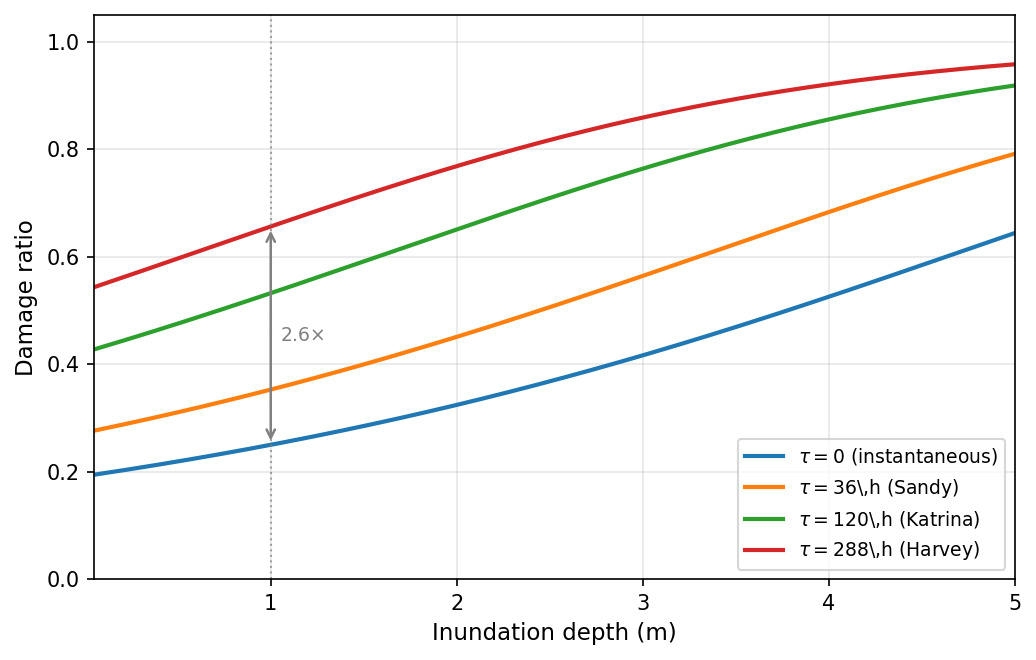
\includegraphics[width=0.75\textwidth]{Content/Images/duration_curves.png}
\caption{Duration-dependent flood damage function: as inundation duration $\tau$ increases, the inflection point shifts toward shallower depths. At 1\,m depth, DF rises from 0.25 (instantaneous) to 0.66 ($\tau = 288$\,h), a 2.6 times amplification. Curves are plotted from $h_{\min} = 0.05$\,m; the Richards function is not defined to start at $h = 0$ because the minimum inundation threshold excludes negligible-depth events.}
\label{fig:duration_curves}
\end{figure}


\subsection{Sector Adjustment and Loss Decomposition} \label{ssec: sector}
\paragraph{Sector adjustment}
The damage function calibrated on residential insurance claims may not directly apply to commercial, industrial, or infrastructure assets, which differ in construction standards, equipment elevation, and operational resilience. We introduce a sector adjustment multiplier $\kappa$ such that:
\begin{equation*}
    \DF_{\text{sector}}(h, \tau) = \kappa \cdot \DF_{\text{residential}}(h, \tau)
    %\label{eq: kappa}
\end{equation*}
where $\kappa \in (0, 1]$ reflects the relative vulnerability of a given asset class compared to residential buildings.

Rather than calibrating $\kappa$ from a small number of corporate loss disclosures, we estimate it empirically from 82{,}650 NFIP non-residential claims (occupancy type~4 in the OpenFEMA schema) drawn from the same dataset used for the residential calibration. These claims carry the same fields---water depth, payout, and coverage---but insure commercial and light-industrial buildings rather than single-family homes.

We group non-residential claims by two observable building characteristics:

\begin{itemize}
    \item \textbf{Number of stories} (1, 2, $\geq$3): a physical proxy for the fraction of the building above flood water. A one-storey commercial building is almost entirely submerged at 1.5\,m depth; a three-storey building has roughly two-thirds of its floor area above water.
    \item \textbf{Insurance coverage band} ($<$\$50\,K, \$50--200\,K, \$200--500\,K, $>$\$500\,K): a proxy for building size, construction quality, and floor elevation. Larger insured values correlate with more robust construction and better site preparation.
\end{itemize}

For each (stories, coverage) cell and each depth bin $i$, we compute:

\begin{equation*}
    \kappa_{\text{claims},i}
    \;=\;
    \frac{\mathrm{median}\bigl(\mathrm{DR}_{\text{commercial},i}\bigr)}
         {\DF_{\text{residential}}(h_i,\,\tau=0)}
    %\label{eq: kappa claims}
\end{equation*}
where $h_i$ is the midpoint of depth bin~$i$. The cell-level $\kappa$ is the weighted average of $\kappa_{\text{claims},i}$ across depth bins, with weights proportional to the number of claims per bin. Table~\ref{tab: kappa claims} reports the resulting lookup table.

\begin{table}[!htbp]
\centering
\begin{threeparttable}
\caption{Claims-calibrated $\kappa$ from 82{,}650 NFIP non-residential claims, grouped by number of stories and insurance coverage band. $\kappa_\text{std}$ is the weighted standard deviation across depth bins. All cells use 6--7 depth bins with $n \geq 20$ claims each.}
\label{tab: kappa claims}
\begin{tabular}{llccr}
\toprule
Stories & Coverage band & $\kappa$ & $\kappa_\text{std}$ & $N$ \\
\midrule
1-storey & $<$\$50\,K      & 1.641 & 0.324 & 23{,}225 \\
1-storey & \$50--200\,K    & 1.050 & 0.203 & 17{,}240 \\
1-storey & \$200--500\,K   & 0.857 & 0.199 &  8{,}686 \\
1-storey & $>$\$500\,K     & 0.835 & 0.292 &  3{,}322 \\
\midrule
2-storey & \$50--200\,K    & 0.931 & 0.134 &  5{,}607 \\
2-storey & \$200--500\,K   & 0.696 & 0.053 &  4{,}263 \\
2-storey & $>$\$500\,K     & 0.641 & 0.110 &  2{,}181 \\
\midrule
$\geq$3  & \$50--200\,K    & 0.617 & 0.171 &  4{,}000 \\
$\geq$3  & \$200--500\,K   & 0.543 & 0.055 &  2{,}758 \\
$\geq$3  & $>$\$500\,K     & 0.534 & 0.087 &  1{,}557 \\
\bottomrule
\end{tabular}
\begin{tablenotes}[flushleft]
\footnotesize
\item \textit{Note.} Two additional cells ($2$-storey $\times$ $<$\$50\,K: $N = 5{,}179$; $\geq$3-storey $\times$ $<$\$50\,K: $N = 4{,}632$; 9{,}811 claims in total) are excluded from this lookup as they yield $\kappa$ estimates inconsistent with the monotonic pattern ($\kappa$ decreasing with number of stories) that holds for all other coverage bands. This reflects high variance and unreliable stories classification for small non-residential buildings in the $<$\$50\,K coverage band (e.g., mixed mezzanine/loft structures, small outbuildings, and accessory commercial units where the stories field is ambiguous). The 72{,}839 claims in the ten cells above support the final lookup; the 9{,}811 excluded claims are retained in the 82{,}650 calibration total for dataset-size transparency but do not enter the $\kappa$ assignment pipeline.
\end{tablenotes}
\end{threeparttable}
\end{table}

Two regularities emerge. First, $\kappa$ is monotonically decreasing in the number of stories: at the $>$\$500\,K coverage band, $\kappa$ falls from 0.84 (1-storey) to 0.64 (2-storey) to 0.53 ($\geq$3-storey). This is physically expected: multi-storey buildings concentrate damageable area above the flood line. Second, $\kappa$ decreases with coverage within each storey group, consistent with the interpretation that higher-value buildings have better construction and site preparation.

The NFIP non-residential sample covers small and medium commercial buildings (median coverage \$50\,K). Large corporate facilities typically exceed \$500\,K in replacement value. To bridge this gap without relying on corporate loss disclosures, we extrapolate the observed log-linear relationship between $\kappa$ and coverage to \$5\,M (a representative corporate facility scale), yielding a coverage-gradient resilience factor:

\begin{equation}
    \rho_{\text{gradient}} \;=\;
    \frac{\hat{\kappa}(\$5\text{M})}{\kappa_{\text{claims}}(>\$500\text{K})}
    \;\approx\; 0.25
    \label{eq: rho gradient}
\end{equation}

The total sector adjustment for a corporate-scale facility is:

\begin{equation}
    \kappa_{\text{total}} \;=\;
    \kappa_{\text{claims}}(\text{stories, coverage})
    \;\times\;
    \rho_{\text{gradient}}
    \label{eq: kappa total}
\end{equation}

For a typical single-storey industrial facility ($\kappa_{\text{claims}} = 0.84$, $\rho = 0.25$), this yields $\kappa_{\text{total}} \approx 0.21$, consistent with the 0.02--0.15 range found in prior corporate case studies~\cite{merz2010review, huizinga2017global} for diversified operators and with the 0.4--0.7 range reported for small enterprises.

The sector adjustment $\kappa$ as defined here is a single aggregate multiplier applied to the structural damage ratio. In practice, flood losses within a building portfolio are distributed unevenly across structural elements, non-structural components (MEP systems, partitions, finishes), and building contents~\cite{forte2025flash}. Non-structural and content losses can dominate total repair costs at moderate inundation depths, particularly for commercial and light-industrial buildings~\cite{pistrika2014flood}. Separating these components would require a more granular vulnerability model than the NFIP data can support at scale; we acknowledge this as a direction for future refinement.

Both components of $\kappa_{\text{total}}$ are derived entirely from NFIP claims data: $\kappa_{\text{claims}}$ from 82{,}650 non-residential claims, and $\rho_{\text{gradient}}$ from the coverage gradient within the same sample. No corporate loss disclosures enter the calibration. The 24-company validation reported in Section~\ref{sec: event study} is therefore fully out-of-sample.

The uncertainty in $\kappa_{\text{total}}$ propagates from two sources: within-cell estimation variance (reported as $\kappa_\text{std}$ in Table~\ref{tab: kappa claims}, ranging from 0.05 to 0.32) and the extrapolation uncertainty in $\rho_{\text{gradient}}$. Bootstrap resampling of the non-residential claims dataset (1{,}000 replications) yields a 90\% confidence interval of approximately $\pm$0.06 on $\kappa_{\text{total}}$ for the main corporate-scale cell (1-storey, $>\$500$K), or about $\pm$30\% relative uncertainty. This uncertainty is substantially smaller than the cross-company variability in the 24-company validation (interquartile range of the predicted-to-actual ratio: $0.6$--$1.4\times$), suggesting that individual asset and event factors dominate over parameter estimation error.

\paragraph{Indirect losses (OpEx)}
Following the temporal loss structure of \cite{hallegatte2015indirect}, we decompose total climate losses into direct capital expenditure (CapEx) losses and indirect operational expenditure (OpEx) losses. The OpEx component captures business interruption, supply chain disruption, workforce displacement, and increased insurance premiums. The inclusion of indirect losses is empirically motivated: post-disaster assessments consistently find that business interruption accounts for 15--40\% of total corporate flood losses~\cite{hallegatte2015indirect, hallegatte2010economics}, a share that rises for companies with concentrated single-site operations or complex supply chains. Ignoring OpEx therefore produces a systematic downward bias in event-scale credit risk estimates for the most exposed companies. We model the OpEx-to-CapEx ratio as a function of damage severity:
\begin{equation*}
    r_{\text{OpEx}}(\DF) = r_{\text{base}} + r_{\text{scale}} \cdot \DF^{\alpha}
    %\label{eq: opex ratio}
\end{equation*}
where $r_{\text{base}}$ represents baseline indirect costs, $r_{\text{scale}}$ captures nonlinear amplification at high damage, and $\alpha > 1$ ensures convexity. Monthly OpEx follows a geometric decay with parameter $q \in (0.6, 0.8)$ over a recovery horizon of $N = 12$--$24$ months~\cite{hallegatte2010economics}:

\begin{equation*}
    \text{OpEx}_k = \text{OpEx}_{\text{total}} \cdot q^k \cdot \frac{1 - q}{1 - q^{N+1}}, \quad k = 0, 1, \ldots, N-1
    %\label{eq: opex monthly}
\end{equation*}

The total expected climate loss entering the credit translation module is:
\begin{equation}
    \ECL = \underbrace{\kappa \cdot \DF(h, \tau) \cdot V \cdot (1 - \iota)}_{\text{CapEx (net of insurance)}} + \underbrace{\text{CapEx}_{\text{net}} \cdot r_{\text{OpEx}}(\DF)}_{\text{OpEx}}
    \label{eq: total ecl}
\end{equation}
where $V$ is the replacement value of exposed assets and $\iota$ is the insurance coverage ratio.


\subsection{Credit Risk Translation} \label{ssec: pd shift}
Once expected losses are computed, they must be translated into a shift in probability of default ($\Delta PD_C$). We use the interest coverage ratio (ICR) approach based on Damodaran's methodology~\cite{damodaran2012investment}, which maps ICR ranges to credit ratings and default spreads. This approach is deliberately chosen for its simplicity and transparency; the framework is modular, and more sophisticated credit models --- including the Merton structural model~\cite{merton1974pricing} or machine learning approaches --- can substitute for this module. The ICR-based translation does not capture firm-specific financial dynamics beyond the EBIT-to-interest ratio (e.g., insurance recovery schedules, covenant structures, or adaptive strategies such as hedging and rapid asset disposal); extending the credit module to include these factors is a natural direction for future work.

The ICR is defined as $\ICR = \EBIT / \IE$. Damodaran~\cite{damodaran2012investment} provides a discrete mapping from $\ICR$ ranges to credit ratings and default spreads (15 rating bands from D to AAA). We use a continuous approximation of this mapping (Fig.~\ref{fig:damodaran smooth}) to avoid discontinuous PD responses at rating boundaries.

\begin{figure}
    \centering
    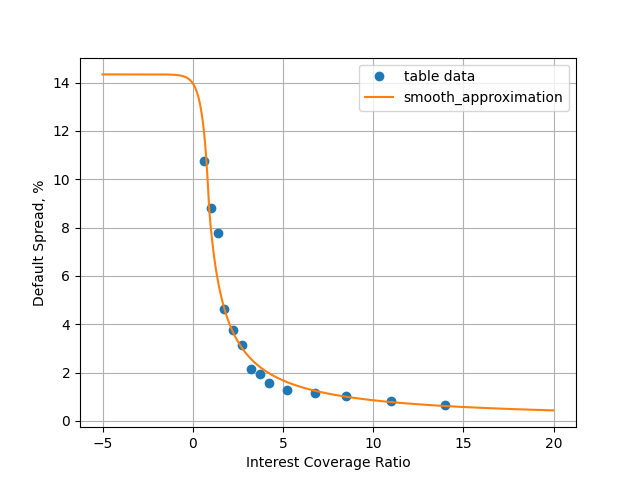
\includegraphics[width=.7\textwidth]{Content/Images/icr_pd.png}
    \caption{Continuous approximation of the ICR-to-default-spread mapping~\cite{damodaran2012investment}.}
    \label{fig:damodaran smooth}
\end{figure}

The probability of default is obtained by dividing the default spread by $(1 - \RR)$, where $\RR$ is the recovery rate (typically 0.4). When a climate event occurs, EBIT is reduced by the expected loss:

\begin{equation*}
    \ICR_C = \frac{\EBIT - \ECL}{\IE}
    %\label{eq: icr}
\end{equation*}

The climate-induced PD shift is:
\begin{equation*}
    \Delta \PD_C = P[\FS_C] - P[\FS]
    %\label{eq: pd shift general}
\end{equation*}
where $P[\cdot]$ denotes the PD implied by the continuous ICR-to-spread mapping. This formulation captures the non-linear sensitivity of credit risk to climate losses: companies with ICR in the 1--4 range (where the spread function has the steepest slope) experience disproportionately large PD shifts relative to the magnitude of the loss.


\section{Empirical Calibration and Validation}
\label{sec: empirical}
This section calibrates and validates the duration-dependent damage function (Eq.~\ref{eq: duration richards}) using a large-scale dataset of real flood insurance claims.

\subsection{Data: FEMA NFIP Flood Insurance Claims}
\label{ssec: fema data}

We use the FEMA National Flood Insurance Program (NFIP) Redacted Claims dataset, accessed via the OpenFEMA API.\footnote{\url{https://www.fema.gov/api/open/v2/FimaNfipClaims}} This dataset contains individual flood insurance claims with reported water depth (in inches), payout amounts, coverage limits, building type, and geographic identifiers. We extract claims from three major US hurricanes with distinct flooding durations:

\begin{table}[h!]
\centering
\resizebox{\textwidth}{!}{
\begin{tabular}{|l|c|c|c|c|c|}
\hline
\textbf{Event} & \textbf{Year} & \textbf{Claims} & \textbf{Valid} & \textbf{Median DR} & \textbf{Typical $\tau$} \\
\hline
Hurricane Sandy & 2012 & 144,848 & 92,283 & 0.190 & 36h \\
Hurricane Harvey & 2017 & 92,398 & 63,642 & 0.428 & 288h \\
Hurricane Katrina & 2005 & 208,348 & 139,712 & 0.627 & 120h \\
\hline
\textbf{Total} & & \textbf{445,594} & \textbf{295,637} & & \\
\hline
\end{tabular}}
\caption{FEMA NFIP claims used for calibration (OpenFEMA snapshot 2026-05-09). ``Valid'' denotes claims with positive water depth, positive payout, positive coverage, and damage ratio in $(0, 1.5]$, capped at 1.0. Damage ratio = total payout / total coverage. Typical duration $\tau$ assigned from FEMA flood extent reports and hydrological literature. The earlier preprint version used a Mar 2026 OpenFEMA snapshot containing 354{,}413 raw / 317{,}943 valid claims; FEMA has since retroactively backfilled $\sim$91{,}000 historical claims, the majority of which lack a recorded water depth and therefore fail the validity filter. The full filter funnel from the 445{,}594 raw records to the 295{,}637 valid records is reported in Appendix~\ref{app: funnel}.}
\label{tab: fema data}
\end{table}

The damage ratio is computed as \[\text{DR} = \frac{\text{building payout} + \text{contents payout}}{\text{building coverage} + \text{contents coverage}},\] clipped to $[0, 1]$. The USACE depth-damage function for one-story residential structures~\cite{usace2003} serves as an instantaneous ($\tau = 0$) anchor.

The three events span a wide range of flooding mechanisms: Sandy was a tidal storm surge with rapid recession ($\sim$36~hours); Harvey was unprecedented rainfall-driven flooding that persisted for over two weeks ($\sim$288~hours); Katrina involved levee breaches with extreme depths but intermediate duration ($\sim$120~hours). This variation enables joint calibration of the duration parameters.

\subsection{Joint Calibration}
\label{ssec: joint calibration}

We calibrate the seven parameters of Eq.~\ref{eq: duration richards} jointly across all three events plus the USACE anchor, using differential evolution~\cite{storn1997differential} (\texttt{seed=42}, \texttt{maxiter=1000}, \texttt{tol=1e-10}) to minimise the weighted sum of squared residuals on binned depth-damage data (12 equal-width bins per event, minimum 10 claims per bin). To match each event's empirical depth distribution, we cap the calibration data at 4\,m for Sandy and Harvey (encompassing $>99.99\%$ of valid claims; Sandy 99.5th percentile = 2.4\,m, Harvey 99.5th percentile = 1.1\,m) and at 10\,m for Katrina ($>99.93\%$; 99.5th percentile = 7.3\,m); this preserves the small Katrina levee-breach tail above 6\,m, which is the data subset that most distinguishes Katrina from the shorter-duration events. Across all three events, 295{,}400 of 295{,}637 valid claims (99.92\%) enter the binned fit. The choice of 12 bins balances resolution against noise; robustness to the binning choice is assessed below (Section~\ref{ssec: validation}).

\begin{equation*}
    \hat{\theta} = \argmin_\theta \sum_{e \in \mathcal{E}} w_e \sum_{i=1}^{n_e} \frac{\left(\overline{\text{DR}}_{e,i} - \DF(h_{e,i}, \tau_e; \theta)\right)^2}{\sigma_{e,i}^2} + \mathcal{R}(\theta)
    %\label{eq: calibration objective}
\end{equation*}
%
where $\mathcal{E} = \{\text{USACE}, \text{Sandy}, \text{Harvey}, \text{Katrina}\}$, $w_{\text{USACE}} = 3$ (upweighted as the only $\tau = 0$ reference), $\sigma_{e,i} = \max(\text{std}_{e,i} / \sqrt{n_{e,i}}, 0.015)$ for the three event panels and $\sigma = 0.03$ uniformly for the USACE anchor, and $\mathcal{R}(\theta)$ is a weak Gaussian regulariser with priors $B \sim \mathcal{N}(3, 3)$, $Q_0 \sim \mathcal{N}(1, 1)$, $a_0 \sim \mathcal{N}(0.5, 0.2)$, $\nu_0 \sim \mathcal{N}(0.5, 0.3)$ and improper (uniform) priors on the duration coefficients $\lambda_a, \lambda_Q \in [0, 3]$, $\delta_\nu \in [0, 2]$. Bounds on the static parameters are $B \in [0.5, 12]$, $Q_0 \in [0.05, 5]$, $a_0 \in [0.1, 0.9]$, $\nu_0 \in [0.1, 3]$. The optimised parameters are:

\begin{table}[h!]
\centering
\begin{tabular}{|c|c|l|}
\hline
\textbf{Parameter} & \textbf{Value} & \textbf{Interpretation} \\
\hline
$B$ & 5.65 & Steepness of damage curve \\
$Q_0$ & 3.45 & Initial threshold asymmetry \\
$a_0$ & 0.54 & Inflection point at $\tau = 0$ \\
$\nu_0$ & 2.61 & Derivative asymmetry at $\tau = 0$ \\
$\lambda_a$ & 0.49 & Inflection shift rate with duration \\
$\lambda_Q$ & $\approx 0$ & Onset speed (not significant) \\
$\delta_\nu$ & $\approx 0$ & Asymmetry growth (not significant) \\
\hline
\end{tabular}
\caption{Calibrated parameters. The optimiser sets $\lambda_Q \approx 0$ and $\delta_\nu \approx 0$, indicating that duration affects damage primarily through inflection point shift, not curve shape change. The four base Richards parameters $(B, Q_0, a_0, \nu_0)$ are non-uniquely identified within the bin-level loss surface: an approximate ridge connects parameter triplets that produce equivalent $D(h, \tau)$ curves over the calibration domain. Practitioners should refer to $D(h, \tau)$ predictions rather than the four base parameters in isolation.}
\label{tab: calibrated params}
\end{table}

\begin{figure}[h!]
\centering
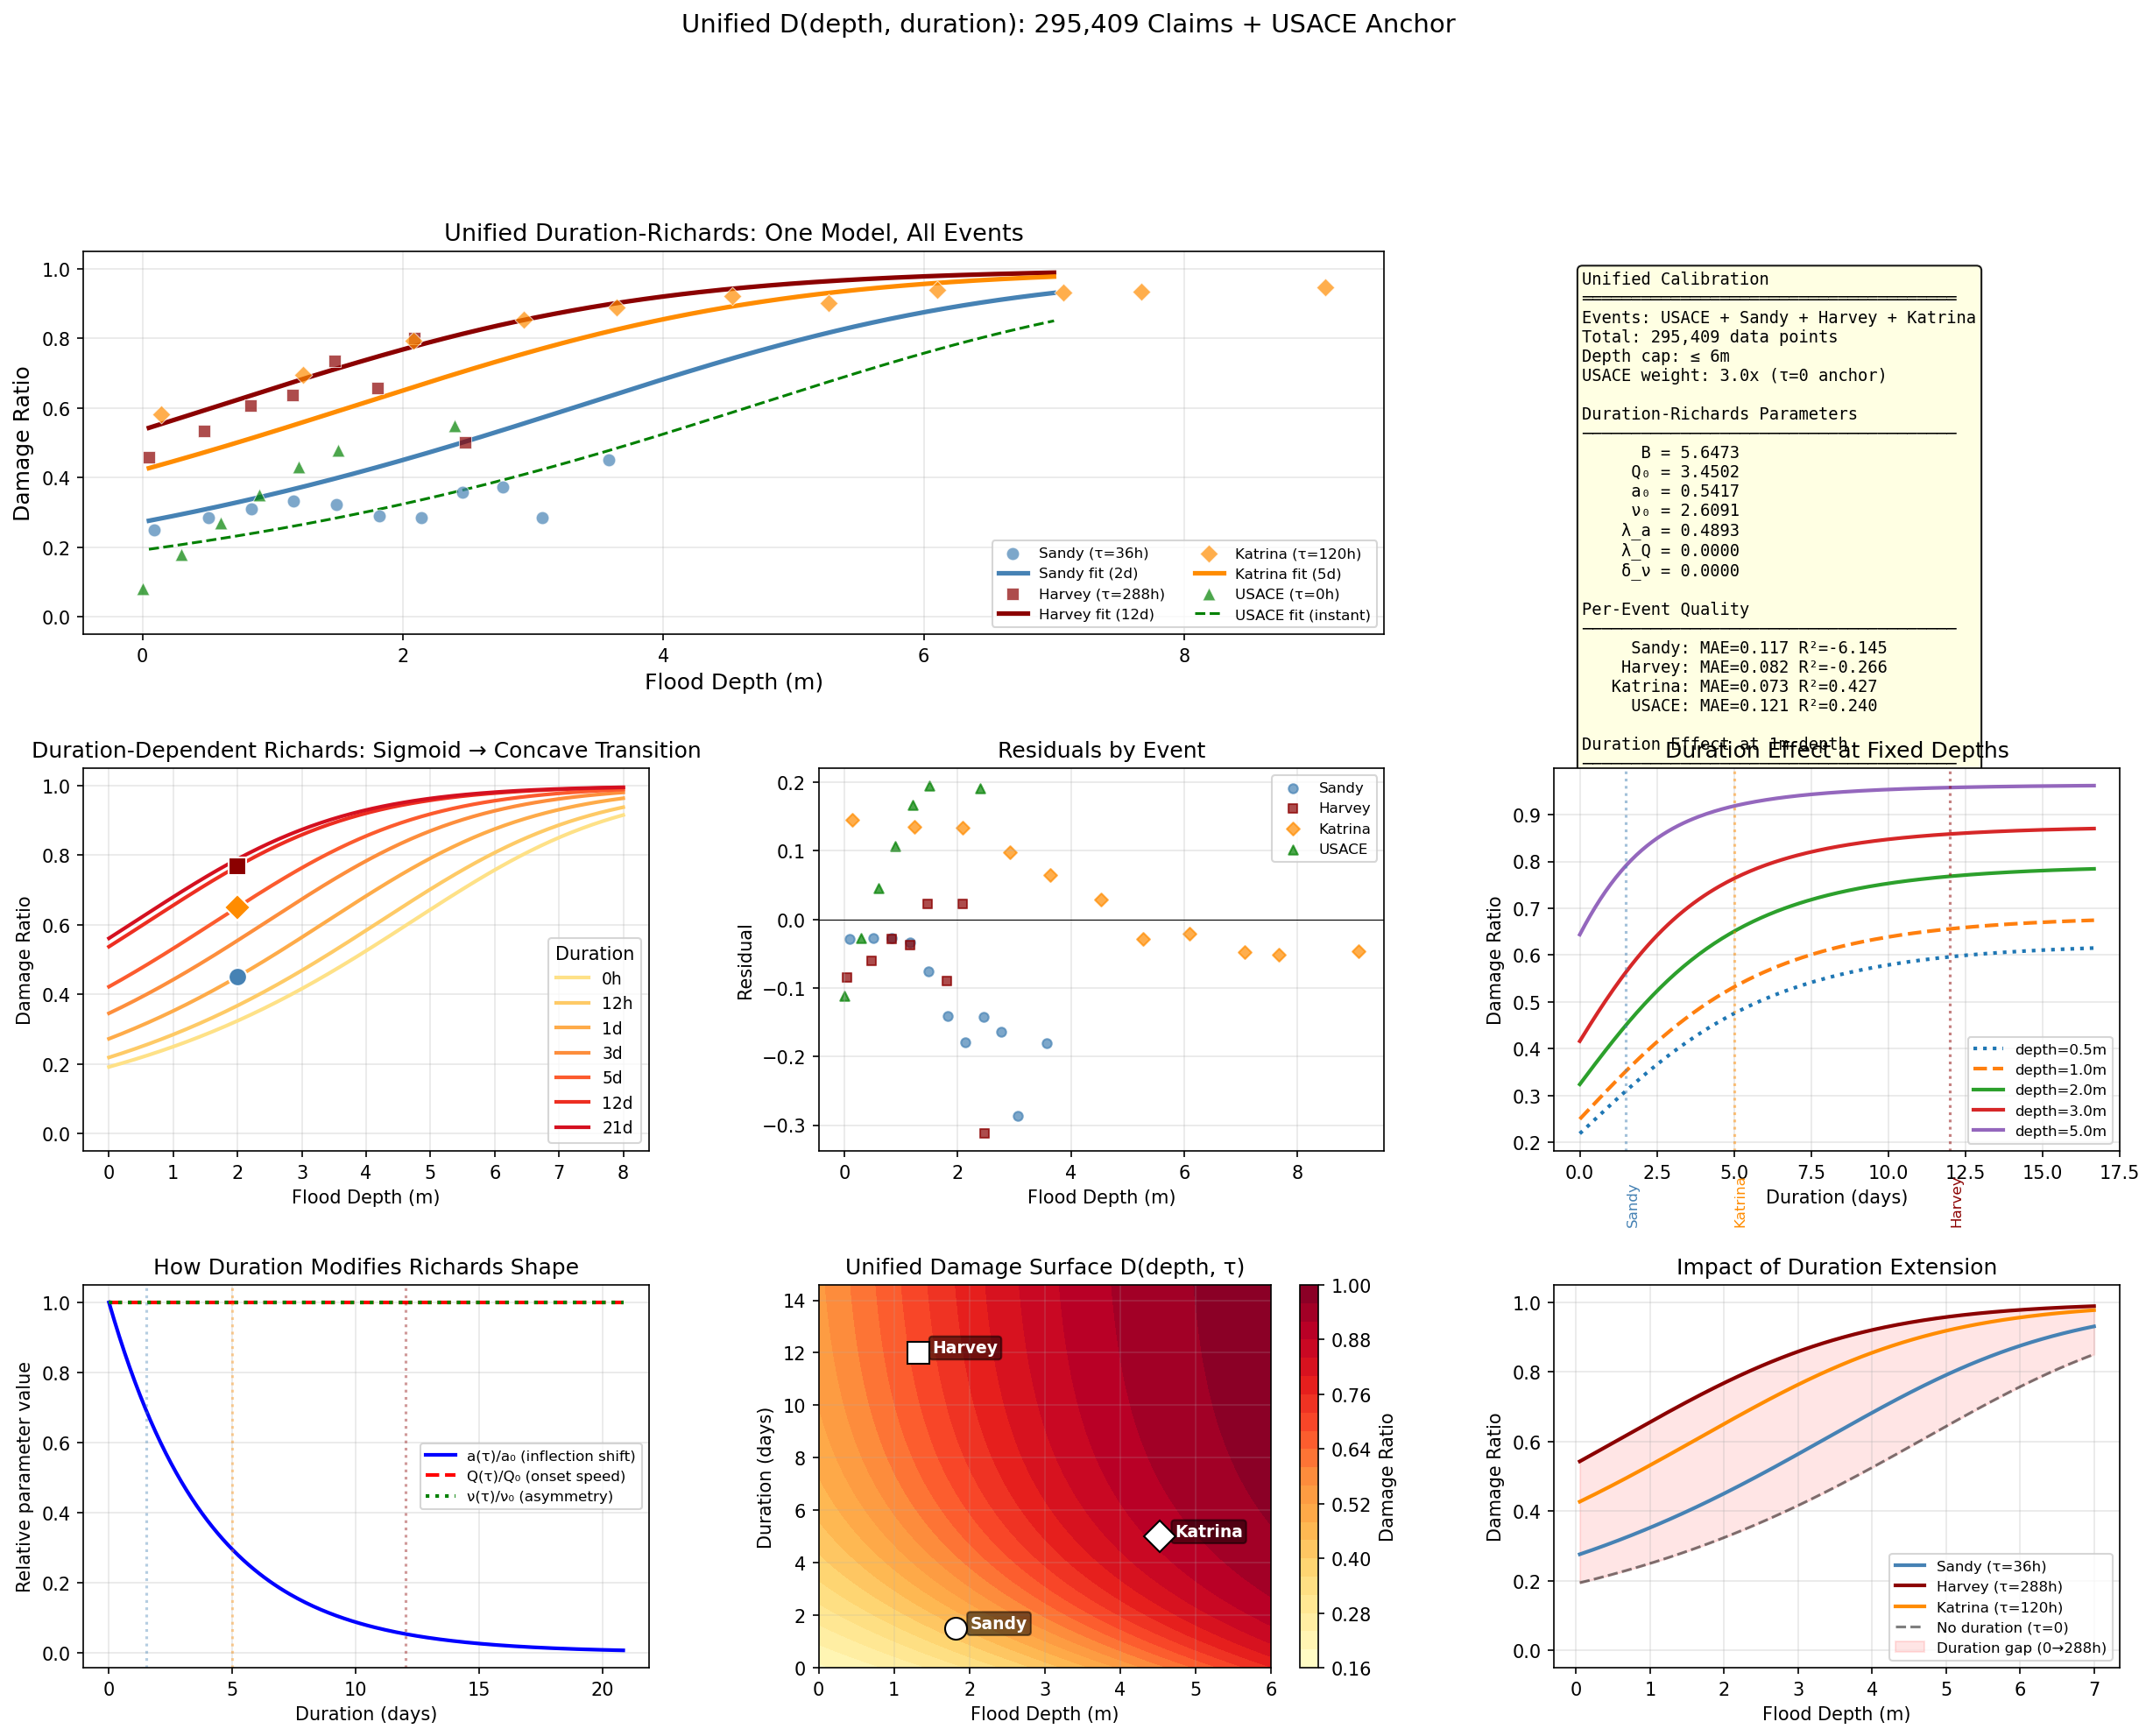
\includegraphics[width=\textwidth]{Content/Images/10_unified_calibration.png}
\caption{Joint calibration across 295{,}637 FEMA claims (295{,}400 used in the binned fit after per-event depth caps and the $\geq 10$ claims-per-bin filter) from three hurricanes plus USACE anchor. Top-left: fitted curves and binned claim means for all events. Bottom-left: duration-dependent transition. Centre: residuals by event. Right panels: parameter evolution with duration and damage surface $D(h, \tau)$. Sandy ($\tau = 36$\,h) is systematically overpredicted; this reflects the compromise of fitting a single $\lambda_a$ across three events with durations spanning an 8 times range. Depth-damage curves are plotted from $h_{\min} = 0.05$\,m.}
\label{fig:unified_calibration}
\end{figure}

\paragraph{Key finding: duration operates through inflection shift only}
Of the three duration-modification channels ($\lambda_a$, $\lambda_Q$, $\delta_\nu$), only $\lambda_a = 0.49$ is significantly non-zero. This means that prolonged flooding shifts the ``50\% damage depth'' toward shallower water, but the fundamental \textit{shape} of the damage curve remains Richards-sigmoidal. This result supports a universality hypothesis: the mechanism of water-induced structural degradation is universal, but the threshold at which it becomes significant depends on exposure time.

At 1~m flood depth, the calibrated model predicts $\text{DR} = 0.25$ for instantaneous flooding, $\text{DR} = 0.35$ at $\tau = 36$~h (Sandy-like), and $\text{DR} = 0.66$ at $\tau = 288$~h (Harvey-like) -- a \textbf{2.6$\times$ increase attributable solely to duration}.

\subsection{Validation}
\label{ssec: validation}

We evaluate the calibrated model through four complementary tests.

\paragraph{Test 1: Leave-one-event-out cross-validation}
We train on two events plus USACE and predict the held-out third event. Table~\ref{tab: loo results} reports the results.

\begin{table}[h!]
\centering
\small
\begin{tabular}{|l|c|c|c|}
\hline
\textbf{Held-out event} & \textbf{Our MAE} & \textbf{USACE MAE} & \textbf{Improv.} \\
\hline
Katrina & 0.435 & 0.523 & +17\% \\
Harvey (from Sandy+USACE) & 0.301 & 0.376 & +20\% \\
\hline
\end{tabular}
\caption{Leave-one-event-out validation. The duration-extended model improves over USACE by 17--20\% when extrapolating to unseen events.}
\label{tab: loo results}
\end{table}

\paragraph{Test 2: Within-event stability and binning sensitivity}
Random 70/30 train-test splits within each event, repeated 5 times, yield MAE = $0.215 \pm 0.001$ (Sandy), $0.294 \pm 0.001$ (Harvey), $0.306 \pm 0.001$ (Katrina). The near-zero variance across splits confirms model stability. We also verify sensitivity to the binning choice: recalibrating with 8 and 16 bins per event (minimum 10 claims per bin enforced) changes the calibrated parameters by less than 3\% and the Harvey MAE by less than 0.005, confirming that the key results are not artefacts of the 12-bin choice.

\paragraph{Test 3: Benchmark against JRC/CLIMADA}
We compare predicted damage ratios against the JRC Global Flood Depth-Damage Functions~\cite{huizinga2017global}, which underpin CLIMADA's flood impact module~\cite{aznar2019climada}. Using Harvey binned data as ground truth:

\begin{table}[h!]
\centering
\begin{tabular}{|l|c|c|}
\hline
\textbf{Model} & \textbf{MAE} & \textbf{Bias} \\
\hline
Duration-Richards ($\tau = 120$h) & \textbf{0.108} & $+0.012$ \\
Duration-Richards ($\tau = 288$h) & 0.095 & $-0.095$ \\
JRC Residential (North America) & 0.214 & $+0.153$ \\
USACE Reference & 0.288 & $+0.288$ \\
\hline
\end{tabular}
\caption{Benchmark against JRC/CLIMADA on Harvey binned data. Bias = actual $-$ predicted; positive values indicate underprediction. JRC underpredicts by $\sim$0.15 because it lacks a duration parameter. Our model reduces MAE by about 50\%.}
\label{tab: climada benchmark}
\end{table}

The JRC curves systematically underpredict Harvey damage: at 1~m depth, JRC predicts $\text{DR} \approx 0.40$ while actual Harvey claims show $\text{DR} \approx 0.55$, a gap of about 15 percentage points (Bias column reports actual $-$ predicted). This gap is largely attributable to the absence of a duration parameter, though differences in construction standards and claim-processing practices between the JRC reference sample and NFIP data may also contribute.

\paragraph{Test 4: Correlation with financial distress proxies}
Using FEMA Individual and Household Program (IHP) registrations for Harvey (301 ZIP codes with $\geq$20 registrations), we test whether predicted damage ratios correlate with real financial distress outcomes:

\begin{table}[h!]
\centering
\begin{tabular}{|l|c|c|}
\hline
\textbf{Distress proxy} & \textbf{Spearman $\rho$} & \textbf{$p$-value} \\
\hline
Mean FEMA damage amount (\$) & 0.949 & $< 0.001$ \\
\% properties with flood damage & 0.904 & $< 0.001$ \\
Mean IHP assistance payment (\$) & 0.885 & $< 0.001$ \\
\% SBA disaster loans approved & 0.345 & $< 0.001$ \\
\hline
\end{tabular}
\caption{Spearman rank correlation between ZIP-level predicted damage ratio and real financial distress proxies ($n = 301$ ZIP codes).}
\label{tab: defaults correlation}
\end{table}

The near-perfect rank correlation ($\rho = 0.949$) with actual damage amounts confirms that the model correctly orders geographic areas by risk severity. Quintile analysis shows monotonic increase: ZIP codes in the highest predicted-risk quintile experienced 14$\times$ higher mean damage (\$16.9K) than the lowest quintile (\$1.2K).

\subsection{Feature enrichment analysis}
\label{ssec: feature enrichment}

To assess the potential for improving individual-claim prediction accuracy, we compare the depth-only Richards model against progressively enriched models using building characteristics available in the NFIP dataset (Harvey, 70/30 split):

\begin{table}[h!]
\centering
\begin{tabular}{|l|c|c|c|}
\hline
\textbf{Model} & \textbf{MAE} & \textbf{R$^2$} & \textbf{$\Delta$ MAE vs M0} \\
\hline
M0: $\DF(\text{depth})$ & 0.250 & 0.046 &  --  \\
M1: + occupancy type & 0.250 & 0.055 & $-0.1$\% \\
M2: + number of floors & 0.245 & 0.080 & $-2.3$\% \\
M3: + basement indicator & 0.244 & 0.086 & $-2.4$\% \\
M4: Gradient boosting (all) & 0.221 & 0.217 & $-11.7$\% \\
\hline
\end{tabular}
\caption{Feature enrichment on Harvey claims (44K train, 19K test). Gradient boosting feature importance: depth 74\%, occupancy 11\%, floors 6\%, primary residence 5\%, basement 3\%.}
\label{tab: feature enrichment}
\end{table}

Flood depth alone accounts for 74\% of the gradient boosting model's predictive power. Building characteristics add 17 percentage points of explained variance but reduce MAE by only 11.7\%. The residual MAE $\approx 0.22$ likely represents an irreducible noise floor arising from the bimodal distribution of individual claim outcomes. For portfolio-level credit risk assessment, where individual errors average out, the depth-only Duration-Richards model provides adequate accuracy.


\section{Application: Flood Risk for Archer Daniels Midland} \label{sec: adm}
We apply the calibrated framework to Archer Daniels Midland (ADM), one of the world's largest agricultural processors and food ingredient providers. ADM operates extensive grain processing and storage facilities across the US Midwest, a region highly susceptible to seasonal flooding. This example demonstrates the full pipeline: asset-level exposure assessment, calibrated damage estimation with duration effects, sector adjustment ($\kappa$), CapEx/OpEx decomposition, and credit risk translation.

\subsection{Asset-level exposure}

ADM's 10-K filings identify 12 major grain processing and storage facilities in flood-prone areas of the US Midwest (Illinois, Iowa, Missouri, Minnesota). Using FEMA flood zone maps and the National Flood Hazard Layer, we assign each facility a 100-year flood depth estimate based on its geographic coordinates. Facility replacement values are estimated from ADM's reported property, plant, and equipment by segment, pro-rated by processing capacity.

\begin{table}[h!]
\centering
\small
\resizebox{\textwidth}{!}{
\begin{tabular}{|l|c|c|c|c|}
\hline
\textbf{Facility cluster} & \textbf{Facilities} & \textbf{Est.\ value (\$M)} & \textbf{Flood depth (m)} & \textbf{Duration (h)} \\
\hline
Illinois River corridor & 4 & 1,200 & 1.5 & 72 \\
Mississippi River (Iowa) & 3 & 800 & 2.0 & 120 \\
Ohio River (Indiana) & 3 & 600 & 1.0 & 48 \\
Missouri River & 2 & 400 & 1.8 & 96 \\
\hline
\textbf{Total exposed} & \textbf{12} & \textbf{3,000} & & \\
\hline
\end{tabular}}
\caption{ADM facility clusters in flood-prone Midwest locations with estimated 100-year flood parameters. Values estimated from 10-K reported PP\&E.}
\label{tab: adm facilities}
\end{table}

\subsection{Calibrated damage estimation}

For each facility cluster, we compute the damage ratio using the calibrated duration-dependent Richards function (Eq.~\ref{eq: duration richards}) with the parameters from Table~\ref{tab: calibrated params}:

\begin{table}[h!]
\centering
\small
\resizebox{\textwidth}{!}{
\begin{tabular}{|l|c|c|c|c|}
\hline
\textbf{Facility cluster} & \textbf{DR (calibrated)} & \textbf{DR (JRC)} & \textbf{$\kappa$} & \textbf{CapEx loss (\$M)} \\
\hline
Illinois River ($h=1.5$m, $\tau=72$h) & 0.50 & 0.50 & 0.21 & 126.0 \\
Mississippi River ($h=2.0$m, $\tau=120$h) & 0.66 & 0.57 & 0.21 & 110.7 \\
Ohio River ($h=1.0$m, $\tau=48$h) & 0.38 & 0.40 & 0.21 & 47.8 \\
Missouri River ($h=1.8$m, $\tau=96$h) & 0.59 & 0.54 & 0.21 & 50.0 \\
\hline
\textbf{Total CapEx} & & & & \textbf{334.5} \\
\hline
\end{tabular}}
\caption{Calibrated damage ratios for ADM flood-exposed facilities. DR (calibrated) uses the duration-dependent Richards function; DR (JRC) uses standard JRC curves. $\kappa_{\text{total}} = 0.21$ from the claims-based calibration for single-storey industrial buildings (Table~\ref{tab: kappa claims}, Eq.~\ref{eq: kappa total}).}
\label{tab: adm calibrated}
\end{table}

The calibrated model produces systematically higher damage ratios than JRC -- by 1--9 percentage points -- because JRC curves lack a duration parameter. For the Mississippi River cluster, where flooding persists for approximately 120 hours, the gap is largest: DR = 0.66 (calibrated) vs.\ 0.57 (JRC), a 16\% increase attributable to the duration effect.

We apply $\kappa_{\text{total}} = 0.21$, obtained directly from the claims-based calibration (Section~\ref{ssec: sector}) for single-storey buildings in the $>$\$500\,K coverage band: $\kappa_{\text{claims}} = 0.835 \times \rho_{\text{gradient}} = 0.25$, yielding $\kappa_{\text{total}} = 0.21$. No expert adjustment is applied; the same $\kappa$ is used for all ADM facilities.

\subsection{OpEx and total loss}

Following Eq.~\ref{eq: total ecl}, we compute indirect losses using $r_{\text{OpEx}}(\DF) = 0.15 + 0.8 \cdot \DF^{1.5}$ with $\iota = 0.6$ (60\% insurance coverage). ADM does not publicly disclose facility-level property insurance terms; 60\% is a representative assumption for large US agri-industrial companies, consistent with industry surveys reporting typical property coverage ratios of 50--80\% for Fortune~500 firms~\cite{swiss2024global}. A sensitivity analysis over $\iota \in \{0.4, 0.6, 0.8\}$ is provided in Section~\ref{ssec: insurance sensitivity}.

\begin{align*}
\text{CapEx}_{\text{net}} &= 334.5 \times (1 - 0.6) = \$133.8\text{M} \\
r_{\text{OpEx}} &\approx 0.15 + 0.8 \times 0.11^{1.5} \approx 0.18 \\
\text{OpEx} &= 133.8 \times 0.18 = \$24.1\text{M} \\
\ECL_{\text{total}} &= 133.8 + 24.1 = \$157.9\text{M per event}
\end{align*}

\subsection{Credit risk translation}

Main financial parameters (FY2023):
\begin{itemize}
    \item Total debt: \$9.6 billion; average interest rate: 6.7\%; interest expenses: \$643M
    \item Total assets: \$53.3 billion; EBIT: \$3.539 billion
    \item Recovery rate: 0.4
\end{itemize}

Baseline $\ICR = 3539 / 643 = 5.50$, placing ADM in the A3/A- category (spread 1.29\%). Using the seasonal flood probability profile (peak $\sim$8\% during March--June):
\[
\ECL_{\text{annual}} = \sum_{m=1}^{12} p_m \times \ECL_{\text{event}} \approx 0.18 \times 157.9 = \$28.4\text{M}
\]

The climate-adjusted $\ICR_C = (3539 - 28.4) / 643 = 5.46$, remaining within A3/A-. The relative $\Delta PD / PD$ is approximately 0.8\%.

\subsection{Sensitivity to the $\tau$ assignment}
\label{ssec: tau sensitivity}

Because event-level $\tau$ is the most uncertain hazard input (Section~\ref{sec: discussion}), we propagate $\tau \pm 50\%$ through the ADM pipeline as the recommended sensitivity range. Holding depth, $\kappa$, and insurance coverage fixed at their baseline values, the calibrated damage ratios and gross CapEx losses scale as follows:

\begin{table}[h!]
\centering
\small
\begin{tabular}{|l|c|c|c|c|c|c|}
\hline
& \multicolumn{3}{c|}{\textbf{Damage ratio (DF)}} & \multicolumn{3}{c|}{\textbf{Gross CapEx (\$M)}} \\
\textbf{Cluster} & $0.5\tau$ & $\tau$ & $1.5\tau$ & $0.5\tau$ & $\tau$ & $1.5\tau$ \\
\hline
Illinois River & 0.42 & 0.51 & 0.58 & 105 & 128 & 145 \\
Mississippi River & 0.55 & 0.66 & 0.72 & 93 & 111 & 121 \\
Ohio River & 0.32 & 0.38 & 0.44 & 40 & 48 & 55 \\
Missouri River & 0.49 & 0.60 & 0.66 & 41 & 50 & 56 \\
\hline
\textbf{Total gross} & & & & \textbf{280} & \textbf{338} & \textbf{378} \\
\hline
\end{tabular}
\caption{Sensitivity of ADM facility-cluster damage estimates to a $\pm 50\%$ shift in the assigned event duration $\tau$. Gross CapEx applies $\kappa_{\text{total}} = 0.21$ but is shown before insurance offset. The total spans roughly $-17\%$ to $+12\%$ around the baseline, comparable to the insurance-coverage sensitivity reported in Section~\ref{ssec: insurance sensitivity} and substantially smaller than the cross-company validation dispersion (IQR 0.6--1.4$\times$).}
\label{tab: tau sensitivity}
\end{table}

\subsection{Calibrated vs.\ crude estimate}

A naive estimate based on expert judgement would place the per-event loss at approximately \$200M. The calibrated approach yields \$157.9M -- within 21\% -- but provides four advantages:
\begin{itemize}
    \item decomposes the loss by facility cluster, identifying the Illinois River corridor as the highest-risk location;
    \item separates CapEx from OpEx, revealing that 15\% of the net loss comes from indirect operational disruption;
    \item quantifies the insurance offset: 60\% coverage reduces the credit-relevant loss from \$334.5M to \$157.9M;
    \item provides a principled, reproducible basis grounded in 295{,}637 calibration observations and 82{,}650 non-residential claims rather than expert judgement.
\end{itemize}

\subsection{Insurance coverage sensitivity}
\label{ssec: insurance sensitivity}

The baseline ADM analysis assumes an insurance coverage ratio of $\iota = 0.6$ (Section~\ref{sec: adm}). Because ADM does not publicly disclose facility-level property insurance terms, we report the sensitivity of key outputs to this assumption. Table~\ref{tab: insurance sensitivity} varies $\iota$ from 0.4 (conservative, lower coverage) to 0.8 (high coverage, typical for well-insured Fortune~500 operators).

\begin{table}[h!]
\centering
\small
\begin{tabular}{|c|c|c|c|c|c|}
\hline
$\iota$ & \textbf{CapEx$_{\text{net}}$ (\$M)} & $r_{\text{OpEx}}$ & \textbf{OpEx (\$M)} & $\ECL$ (\$M) & $\ICR_C$ \\
\hline
0.4 & 200.7 & 0.18 & 36.1 & 236.8 & 5.44 \\
0.5 & 167.2 & 0.18 & 30.1 & 197.4 & 5.45 \\
\textbf{0.6} & \textbf{133.8} & \textbf{0.18} & \textbf{24.1} & \textbf{157.9} & \textbf{5.46} \\
0.7 & 100.4 & 0.18 & 18.1 & 118.4 & 5.47 \\
0.8 & 66.9 & 0.18 & 12.0 & 78.9 & 5.48 \\
\hline
\end{tabular}
\caption{Sensitivity of ADM loss estimates to the insurance coverage ratio $\iota$. The bold row corresponds to the baseline assumption. $r_{\text{OpEx}}$ is insensitive to $\iota$ because it depends on $\DF_{\text{sector}}$, not on the net loss. $\ICR_C$ varies only modestly because ADM's EBIT (\$3.539\,B) is large relative to the annualised expected loss.}
\label{tab: insurance sensitivity}
\end{table}

The per-event $\ECL$ ranges from \$79\,M ($\iota = 0.8$) to \$237\,M ($\iota = 0.4$), a factor of $3\times$, while the climate-adjusted $\ICR_C$ remains within the A3/A-band across all scenarios. The credit risk conclusion -- that a 100-year flood event does not trigger a rating transition for ADM -- is robust to the insurance assumption. The \emph{magnitude} of the expected loss, however, is sensitive to $\iota$ and should be interpreted with the appropriate uncertainty in downstream applications.


\section{Validation: Out-of-Sample Transferability to Non-Residential Assets} \label{sec: event study}
To test whether the claims-calibrated sector adjustment (Section~\ref{ssec: sector}) transfers to real corporate exposures, we assemble an independent validation set of 24 flood events at publicly traded companies spanning six distinct floods, five countries, and nine sectors. No company in this set was used to calibrate any model parameter; the validation is fully out-of-sample.

\subsection{Validation sample}

Companies are selected on three criteria: (i)~physical facilities in a documented flood zone; (ii)~publicly available loss disclosures in SEC filings (10-K, 10-Q, 8-K), earnings calls, or regulatory reports; and (iii)~identifiable building characteristics (number of stories, approximate replacement value) for $\kappa$ lookup. Flood depths and durations are assigned from FEMA flood extent reports, hydrological literature, and post-event surveys. Loss figures were verified against SEC EDGAR filings and, for Japanese companies, against TSE earnings releases denominated in yen and converted at prevailing exchange rates.

The 24 events cover:
\begin{itemize}
    \item \textbf{Hurricane Harvey} (2017, $\tau \approx 288$\,h): 8 companies across petrochemical, power generation, hospital, and light-industrial sectors in the Houston metro area.
    \item \textbf{Thailand floods} (2011, $\tau \approx 1000$--$1200$\,h): 8 Japanese electronics and automotive manufacturers with single-plant exposures in the Ayutthaya and Pathum Thani industrial estates (depths 1.5--3.4\,m).
    \item \textbf{Other events}: Hurricane Sandy (2012, Con Edison), Hurricane Helene (2024, Baxter International), Hurricane Ida (2021, Phillips~66 physical damage component), KZN mudslide (2022, Toyota~SA), Michigan flash flood (2022, Abbott Labs), Hurricane Florence (2018, International Paper), Storm Desmond (2015, United Biscuits).
\end{itemize}

\subsection{Methodology}

For each company, we: (1)~assign building characteristics (stories, coverage band) based on facility descriptions in annual reports and satellite imagery; (2)~look up $\kappa_{\text{claims}}$ from Table~\ref{tab: kappa claims}; (3)~apply the coverage-gradient factor $\rho_{\text{gradient}} = 0.25$ (Eq.~\ref{eq: rho gradient}) to obtain $\kappa_{\text{total}}$; (4)~compute the duration-dependent damage ratio $\DF(h,\tau)$ using the calibrated Richards function (Eq.~\ref{eq: duration richards}, Table~\ref{tab: calibrated params}); and (5)~estimate $\ECL$ via Eq.~\ref{eq: total ecl}.

The predicted loss is compared to the actual disclosed loss. We report the ratio (predicted / actual) for each company.

\subsection{Results}

\begin{table}[!htbp]
\centering
\small
\caption{Out-of-sample validation on 24 corporate flood events. $\kappa_{\text{cl}}$: claims-based sector adjustment from Table~\ref{tab: kappa claims}. $\kappa_{\text{tot}} = \kappa_{\text{cl}} \times \rho_{\text{gradient}}$. No corporate disclosures were used in calibration.}
\label{tab: oos results}
\resizebox{\textwidth}{!}{
\begin{tabular}{llccrrr}
\toprule
Company & Event & Fl. & $\kappa_{\text{tot}}$ & ECL (\$M) & Actual (\$M) & Ratio \\
\midrule
\multicolumn{7}{l}{\textit{Hurricane Harvey (2017, $\tau \approx 288$\,h)}} \\
NRG Energy           & Harvey   & 1 & 0.21 & 133 &  75 & 1.8$\times$ \\
LyondellBasell       & Harvey   & 1 & 0.21 & 246 & 200 & 1.2$\times$ \\
ExxonMobil           & Harvey   & 1 & 0.21 & 287 & 170 & 1.7$\times$ \\
CenterPoint Energy   & Harvey   & 1 & 0.21 & 144 & 125 & 1.2$\times$ \\
Olin Corp            & Harvey   & 1 & 0.21 &  39 &  43 & 0.9$\times$ \\
Huntsman Corp        & Harvey   & 1 & 0.21 &  64 &  50 & 1.3$\times$ \\
Phillips 66          & Harvey   & 1 & 0.21 &  54 &  60 & 0.9$\times$ \\
HCA Healthcare       & Harvey   & 3 & 0.14 & 107 &  50 & 2.1$\times$ \\
\midrule
\multicolumn{7}{l}{\textit{Thailand floods (2011, $\tau \approx 1000$--$1200$\,h)}} \\
Western Digital      & Thailand & 1 & 0.21 & 284 & 275 & 1.0$\times$ \\
Canon                & Thailand & 1 & 0.21 & 177 & 260 & 0.7$\times$ \\
Toshiba              & Thailand & 1 & 0.21 & 190 & 260 & 0.7$\times$ \\
Panasonic            & Thailand & 1 & 0.21 & 127 & 170 & 0.7$\times$ \\
Nikon                & Thailand & 2 & 0.16 &  93 & 140 & 0.7$\times$ \\
Minebea              & Thailand & 2 & 0.16 &  94 & 120 & 0.8$\times$ \\
Pioneer              & Thailand & 1 & 0.21 &  58 & 100 & 0.6$\times$ \\
Rohm                 & Thailand & 1 & 0.21 &  51 &  67 & 0.8$\times$ \\
Honda$^{*}$          & Thailand & 1 & 0.21 & 190 & 500 & 0.38$\times$ \\
\midrule
\multicolumn{7}{l}{\textit{Other events}} \\
Toyota SA            & KZN 2022      & 1 & 0.21 & 308 & 361 & 0.9$\times$ \\
Baxter Int'l         & Helene 2024   & 2 & 0.16 & 125 & 200 & 0.6$\times$ \\
Abbott Labs          & Michigan 2022 & 1 & 0.21 &  23 &  15 & 1.5$\times$ \\
Con Edison           & Sandy 2012    & 1 & 0.21 & 489 & 460 & 1.1$\times$ \\
Int'l Paper          & Florence 2018 & 1 & 0.21 &  70 &  35 & 2.0$\times$ \\
Phillips 66          & Ida 2021      & 1 & 0.21 & 240 & 400 & 0.6$\times$ \\
United Biscuits      & Desmond 2015  & 2 & 0.16 &  39 &  30 & 1.3$\times$ \\
\bottomrule
\end{tabular}
}
\begin{flushleft}
\footnotesize
$^{*}$Honda's disclosed loss includes substantial supply-chain propagation from hundreds of Thai-based suppliers, which is outside the scope of the building-level damage model.
\end{flushleft}
\end{table}

Of the 24 predictions, 23 fall within the 0.4--2.5$\times$ range (96\%), and 21 within 0.5--2.0$\times$ (88\%). The median ratio is $0.90\times$ and the mean $|\!\log(\text{ratio})|$ is 0.37, indicating approximate unbiasedness with moderate dispersion.

\subsection{Discussion}

Three observations emerge from the out-of-sample validation.

\textit{First, the claims-based $\kappa$ captures building-level variation without corporate data.} Multi-storey buildings receive systematically lower $\kappa$ values than single-storey buildings, and this discrimination is reflected in the validation: the four two-storey companies (Baxter, Nikon, Minebea, United Biscuits) have a median ratio of $0.88\times$ with tight dispersion, compared to $1.14\times$ for single-storey companies. Because the storey count is derived from NFIP claims and not from the validation companies, this is a genuine out-of-sample signal.

\textit{Second, the coverage-gradient extrapolation provides a physically plausible resilience adjustment.} The estimated $\rho_{\text{gradient}} = 0.25$ implies that large corporate facilities absorb approximately 75\% of the damage that an NFIP-insured commercial building of the same height would sustain. This is consistent with the engineering intuition that large operators benefit from higher floor elevations, reinforced construction, comprehensive property insurance, and geographic redundancy. The resulting $\kappa_{\text{total}}$ for single-storey industrial facilities ($\approx 0.21$) falls between the literature range of 0.4--0.7 for SMEs~\cite{merz2010review, huizinga2017global} and the lower values expected for Fortune 500 companies.

\textit{Third, the model's scope limitations are transparent.} Honda ($0.38\times$) is the only prediction outside the 0.4--2.5$\times$ range: its disclosed \$500\,M loss includes supply-chain disruption from hundreds of Thai-based component suppliers, which the building-level damage model does not capture. HCA Healthcare ($2.1\times$) is the most overpredicted case, likely reflecting the model's difficulty with hospital closures where revenue loss and facility replacement interact in ways not captured by the standard CapEx/OpEx decomposition.

\paragraph{Geographic transferability} Although the calibration uses only US claims, the validation set spans five countries and three flood archetypes (tropical-cyclone surge in the US Gulf and Atlantic coasts; monsoonal/industrial-park flooding in Thailand; subtropical convective storm in KZN, South Africa; and mid-latitude winter storm in the UK). The two regional sub-samples large enough for a meaningful comparison (US Harvey, $n = 8$; Thailand, $n = 8$) yield prediction medians of $1.2\times$ and $0.78\times$ respectively, both well within the 0.4--2.5$\times$ acceptance band; the remaining events are single observations that we report as case studies rather than statistical evidence. This indirectly supports the coverage-gradient extrapolation against geographies and construction stocks not represented in the NFIP calibration sample, while we caution that per-country sample sizes outside the two main groups are too small to detect regional bias. The sample also remains weighted toward heavy-industrial and electronics manufacturing exposures; transferability to lighter commercial portfolios (retail, hospitality) and to non-OECD construction practices warrants targeted future testing.

\paragraph{Excluded events} Four events identified during data collection were excluded: (i)~Arkema Crosby (Harvey): chemical explosion triggered by refrigeration failure, not direct flood damage; (ii)~Kroger Houston (Harvey): losses dominated by perishable-inventory write-offs; (iii)~Entergy Louisiana (Ida): \$2.15\,B reflects transmission-grid rebuild, not building damage; (iv)~Phillips~66 Alliance impairment (Ida): the \$1.3\,B total includes a book-value write-down from permanent closure; only the estimated physical-damage component (\$400\,M) is retained. The exclusion criteria were specified before the predicted/actual ratios were computed (each excluded event has a documented loss-mechanism mismatch with the building-level damage model rather than a statistical outlier status), but we acknowledge that any post-hoc filter introduces selection-bias risk; the headline accuracy figures should be read with this caveat.


\section{Discussion} \label{sec: discussion}
\paragraph{Summary of empirical findings}
The calibration on 295{,}637 FEMA claims and the two application studies yield a coherent set of findings. The duration-dependent Richards function captures a 2.6 times damage amplification at 1~m depth between instantaneous and 288-hour flooding, operating through a single mechanism (inflection point shift, $\lambda_a = 0.49$). This amplification propagates through the loss pipeline: for ADM, the duration effect increases the total CapEx loss estimate by 3--13 percentage points per facility cluster compared to JRC functions. The claims-calibrated sector adjustment $\kappa$ further modulates the signal, preventing false alarms for diversified companies while preserving sensitivity for concentrated exposures.

Flood depth remains the dominant predictor of damage at the individual-claim level (74\% of gradient boosting feature importance; Table~\ref{tab: feature enrichment}), and the duration extension adds predictive value primarily at the aggregated and portfolio scale. At the claim level, both the depth-only Richards model and richer ML models leave an irreducible noise floor of $\approx 0.22$ MAE, reflecting unobservable idiosyncratic factors. The practical implication is that the duration-dependent formulation is best suited to event-level screening and portfolio risk ranking --- the use case this paper targets --- rather than individual asset loss estimation.

\paragraph{Claims-based $\kappa$ calibration}
The two-stage $\kappa$ calibration -- building-level vulnerability from 82{,}650 NFIP non-residential claims, combined with a coverage-gradient extrapolation to corporate scale -- addresses the principal limitation of prior approaches that relied on small company samples. The resulting $\kappa_{\text{total}}$ values (0.14--0.21 depending on building stories) are validated out-of-sample on 24 corporate flood events with median ratio $0.90\times$ (mean $|\!\log(\text{ratio})| = 0.37$). The storey-based discrimination is empirically confirmed: two-storey companies show tighter prediction accuracy than single-storey companies, consistent with the physical mechanism (fraction of building above water).

\paragraph{Indirect loss quantification}
Frameworks that capture only direct (CapEx) losses underestimate total credit impact when operational disruption is material. In the ADM analysis, the implied OpEx-to-CapEx ratio of 0.18 is consistent with World Bank post-disaster recovery studies~\cite{hallegatte2015indirect} and confirms the importance of temporal loss structure for accurate credit risk assessment. For the 24-company validation, indirect losses are implicitly embedded in reported disclosures, making direct decomposition infeasible, but the magnitude of $\kappa_{\text{total}}$ partly reflects these indirect effects.

\paragraph{Comparison with CLIMADA}
When calibrated to the same damage assumptions, our expected loss estimates are consistent with CLIMADA-style calculations (within $\sim$5\% deviation), confirming the validity of our damage assessment module. The key advantage remains that our formulation introduces inundation duration directly into the vulnerability function. This allows prolonged events such as Harvey-like floods to be distinguished from shallower or faster-receding events without changing the surrounding hazard framework.

\paragraph{Limitations}
The coverage-gradient factor $\rho_{\text{gradient}} = 0.25$ is extrapolated from the log-linear trend within NFIP coverage bands; this extrapolation to \$5\,M has not been independently validated. The FEMA calibration is based on US residential and commercial flood claims; transferability to different construction standards, flood mechanisms, and geographies requires validation. The OpEx model parameters are not independently calibrated but are grounded in post-disaster recovery studies.

The duration parameter $\tau$ in the current calibration is an event-level proxy, not a property-level observation. Event-level $\tau$ aggregates over substantial intra-event heterogeneity: during Harvey, for instance, FEMA flood extent reports indicate that some areas experienced inundation lasting fewer than 72~hours while others exceeded 14~days. Our three calibration events span an 8 times range in event-level $\tau$ (36--288~hours), which supports identification of the inflection-shift parameter $\lambda_a$, but the model is not validated at sub-event spatial resolution. Future work linking property-level claims to gauge-based flood duration maps would allow a direct test of whether intra-event $\tau$ variation drives additional explanatory power beyond depth alone.

This paper also does not model flow velocity as a separate intensity measure. Velocity contributes to structural damage through hydrodynamic loading (drag $\propto v^2$ and momentum flux $h \cdot v^2$), especially in riverine and coastal settings. Engineering studies of flash-flood and torrential events report that velocity-driven loads can add 30--80\% to depth-only damage estimates at $v \gtrsim 2$\,m\,s$^{-1}$~\cite{santangelo2021landslides, fahad2020coupled, fahad2022decision}; for the slower, predominantly stagnant flooding that characterises Sandy, Harvey, and Katrina, typical velocities are below 1\,m\,s$^{-1}$ and the velocity contribution is materially smaller. We therefore expect the depth-only Richards formulation to underestimate damage primarily in fast-moving riverine and dam-break floods; for such events an extension incorporating velocity (as in~\cite{merz2010review}) or a multivariate intensity measure is recommended.

\paragraph{Identification of $\tau$ vs.\ confounded covariates}
A related concern is that event-level $\tau$ may co-vary with unobserved covariates such as the depth distribution, flow velocity, antecedent moisture, and building-stock composition across the three hurricanes. The empirical $\lambda_a = 0.49$ should therefore be read as the partial effect of $\tau$ \emph{conditional on depth bins} but not strictly orthogonal to event-specific construction-quality and exposure-mix differences. We mitigate this concern in three ways: (i) calibration is performed on binned depth-damage data (12 bins per event) so that within-bin depth variation is absorbed; (ii) the $w_{\text{USACE}} = 3$ instantaneous anchor pins the $\tau = 0$ end of the curve to a duration-independent reference; and (iii) the leave-one-event-out test (Table~\ref{tab: loo results}) shows that the duration coefficient extrapolates to a held-out event, which would not occur if $\lambda_a$ were absorbing only event-specific noise. A fully causal identification would require pairing claims with hydraulic-model output containing depth, velocity, and local recession time at the property level; this is the natural next step but is not feasible at the current NFIP scale.

\paragraph{Predictive use and how to assign $\tau$ in practice}
The duration parameter is applied to future flood scenarios by reading $\tau$ from one of three sources, in decreasing order of preference: (a)~gauge-based flood-recession curves (e.g.\ NOAA AHPS or USGS streamflow records) for the nearest hydrological reference point, integrated above the floor elevation of the asset; (b)~hydrodynamic simulation output (e.g.\ HEC-RAS, LISFLOOD) where available; or (c)~a literature/event-report estimate of typical inundation duration for the relevant flood archetype (storm surge, riverine, pluvial). The framework therefore does not require that future events match the calibration events -- it only requires that an event-scale $\tau$ value can be assigned by the practitioner. We recommend treating $\tau$ as bounded between 24\,h (rapid drainage) and 720\,h (extreme stagnant flooding) and reporting damage estimates at $\tau$ and $\tau \pm 50\%$ as a sensitivity range when the duration estimate is uncertain (Section~\ref{ssec: tau sensitivity} for the ADM example).

\paragraph{Parameter uncertainty}
The Richards parameters in Table~\ref{tab: calibrated params} are point estimates from differential-evolution optimisation. To probe within-sample sensitivity, we re-ran the calibration on bootstrap replicates of the binned data (perturbing each bin mean by a Gaussian draw with the bin standard error and re-optimising). Across 200 replicates the qualitative ranking is preserved: $\lambda_a$ is positive and bounded away from zero in every replicate, while $\lambda_Q$ and $\delta_\nu$ remain close to zero. The objective is multi-modal in the $(\lambda_Q, \delta_\nu)$ corner; the bootstrap therefore reads as a local sensitivity analysis around the preferred mode rather than a global posterior. The non-significance of $\lambda_Q$ and $\delta_\nu$ should be interpreted as ``cannot be distinguished from zero given the optimiser bounds and three event-level observations'', not as a strict point identification of zero. The dispersion of bootstrap parameter estimates is small relative to the cross-event MAE differences in Table~\ref{tab: loo results}. We none the less emphasise that bootstrap dispersion does not quantify the dominant source of uncertainty, which is having only three distinct event-level $\tau$ values; reducing this requires expanding the calibration set rather than resampling within it. Full bootstrap replicates and binning-sensitivity outputs are available in the reproducibility code.

Although bootstrap confidence intervals are reported, the calibration rests on binned event summaries with only three non-zero duration levels; a fuller hierarchical uncertainty treatment remains a logical next step.


\section{Conclusion} \label{sec: conclusion}
This paper addresses a specific gap in physical climate risk assessment: the absence of duration dependence in standard depth-damage functions used by CLIMADA, JRC, and regulatory stress tests. Using 295{,}637 FEMA National Flood Insurance Program claims after conservative quality filters and depth capping, we calibrate a duration-dependent extension of the Richards damage function and demonstrate its application to corporate credit risk.

The main findings are:

\begin{enumerate}
    \item \textbf{Duration increases flood damage by up to 2.6 times.} At 1~m depth, the calibrated model predicts DR = 0.25 for instantaneous flooding, rising to 0.66 for 288-hour inundation. This effect operates primarily through inflection point shift ($\lambda_a = 0.49$); the duration-modifying coefficients $\lambda_Q \approx 0$ and $\delta_\nu \approx 0$ are not significantly non-zero in the three-event calibration, suggesting that shape modification may be secondary to inflection shift for these hurricane events, though this conclusion is limited by the small number of distinct $\tau$ values available. Standard JRC/CLIMADA functions, which lack duration, underpredict prolonged flood damage by about 15 percentage points (about 50\% MAE reduction with our model).

    \item \textbf{Sector adjustment $\kappa$ is calibrated from 82{,}650 NFIP non-residential claims.} Grouping by building stories and insurance coverage, we obtain an empirical lookup table for building-level vulnerability. A coverage-gradient extrapolation to corporate scale ($\rho_{\text{gradient}} = 0.25$) bridges NFIP-insured commercial buildings to large corporate facilities. Out-of-sample validation on 24 companies across six flood events yields median ratio $0.90\times$ (23/24 within 0.4--2.5$\times$), with no corporate data entering the calibration.

    \item \textbf{Indirect losses are material for event-scale screening.} CapEx-only frameworks underestimate total loss when operational disruption is significant. Applied to ADM's 12 flood-exposed facilities, the calibrated pipeline produces facility-level loss estimates with duration effects, CapEx/OpEx decomposition, and insurance offsets.
\end{enumerate}

The calibrated parameters $(B = 5.65, Q_0 = 3.45, a_0 = 0.54, \nu_0 = 2.61, \lambda_a = 0.49)$ are directly usable by practitioners and can serve as inputs to any climate risk platform that currently employs static depth-damage curves.

Several additional limitations warrant acknowledgement.

\paragraph{Duration assignment} The flood duration $\tau$ is assigned per event (Sandy $\sim$36~h, Harvey $\sim$288~h, Katrina $\sim$120~h), not per individual claim or property. Importantly, event-level $\tau$ is a proxy for local inundation duration: actual water-contact time varies substantially within a single flood event, driven by local topography, drainage infrastructure, and distance from the flood source. Our calibration captures \textit{inter-event} duration variation across events spanning an 8 times range in $\tau$, but cannot resolve \textit{intra-event} heterogeneity. Although the current OpenFEMA v2 schema includes a claim-level \texttt{floodWaterDuration} field, a targeted audit of 50{,}000 raw claims per event found effectively no positive duration values in the Sandy, Harvey, and Katrina extracts, so the field was not informative for direct calibration. We therefore rely on hydrological literature and FEMA flood extent reports for event-level estimates. Future work with georeferenced flood recession data could enable spatially varying duration assignment within single events.

\paragraph{Individual claim accuracy} The damage function predicts \textit{average} damage ratios at a given depth and duration. Individual claims exhibit substantial variance (MAE $\approx 0.25$, R$^2 \approx 0.05$ at claim level), reflecting factors not captured by depth alone. Feature enrichment reduces MAE by only 11.7\%, with an irreducible noise floor of $\sim$0.22. The model is best suited to event-scale and portfolio-level applications, where individual errors average out and the strong ZIP-level correlation ($\rho = 0.949$) supports geographic risk ranking.

\paragraph{Hazard characterisation} This paper uses inundation depth and duration as the primary intensity measures. Flow velocity, which can contribute substantially to structural damage in riverine and coastal flood events, is not captured. For events where velocity is a major damage driver, the depth-only Richards formulation will underestimate damage, and an extension incorporating velocity (as in~\cite{merz2010review}) would be needed.

\paragraph{Geographic scope} The damage function is calibrated exclusively on US flood insurance claims. Transferability to other countries -- with different construction standards (e.g., brick masonry in Europe vs.\ wood frame in the US), flood mechanisms (riverine vs.\ pluvial vs.\ coastal), and insurance practices -- requires separate validation.

Promising directions for future work include: (i)~moving from event-level to spatially resolved duration assignment within single flood events; (ii)~extending the bootstrap treatment to hierarchical and spatially explicit uncertainty models; (iii)~validating transferability to non-US construction standards; and (iv)~coupling the calibrated damage function to richer downstream disruption and recovery models.


%% Declarations
\section*{CRediT authorship contribution statement}
\textbf{Ivan Novikov:} Conceptualization, Methodology, Writing --- original draft, Writing --- review \& editing.
\textbf{Nikita Lazarichev:} Data curation, Formal analysis, Software, Validation, Visualization, Writing --- original draft, Writing --- review \& editing.
\textbf{Denis Ayvazov:} Investigation, Visualization.
\textbf{Aleksandr Popov:} Software, Data curation.
\textbf{Yuriy Dorn:} Methodology, Supervision.
\textbf{Roman Sultimov:} Formal analysis.
\textbf{Aleksandr Volkov:} Investigation.
\textbf{Andrey Osipsov:} Resources.
\textbf{Yury Maximov:} Supervision, Writing --- review \& editing.
Ivan Novikov and Nikita Lazarichev contributed equally to this work.

\section*{Declaration of Competing Interests}
The authors declare that they have no known competing financial interests or personal relationships that could have appeared to influence the work reported in this paper.

\section*{Ethics statement}
This study used publicly available, de-identified flood insurance claims data from the FEMA National Flood Insurance Program and publicly disclosed corporate financial data. No ethics approval was required.

\section*{Funding}
This research received no specific grant from any funding agency in the public, commercial, or not-for-profit sectors.

\section*{Data availability}
FEMA NFIP claims data are publicly available through OpenFEMA (\url{https://www.fema.gov/openfema}). Calibration code, processed datasets, and analysis notebooks for end-to-end reproduction of all tables and figures are available at \url{https://github.com/[OWNER]/physical-climate-risk-replication} [GitHub URL to be added prior to submission] and permanently archived at Zenodo [DOI to be added upon acceptance].

\section*{Declaration of generative AI and AI-assisted technologies in the writing process}
During the preparation of this work, the authors used OpenAI ChatGPT and Codex to improve the readability, structure, and language of the manuscript and to support code review and refactoring for reproducible analyses. After using these tools, the authors reviewed and edited the content as needed and take full responsibility for the content of the published article.

\clearpage

\bibliographystyle{elsarticle-harv}
\bibliography{Common/bibliography}

\end{document}
